\documentclass[final]{beamer}
%\documentclass[10pt, handout]{beamer}
%\mode<presentation>{\usetheme{Berlin}}
%\usepackage[orientation=portrait, size=a0, scale=1.25, debug]{beamerposter}
%\documentclass[a4paper,]{article}
\usepackage[utf8]{inputenc}
\usepackage{multicol}
%\usepackage{hyperref}
\usepackage{graphicx}
\usepackage{color}
\usepackage{framed}
\usepackage{subcaption}
\usepackage{float}
\graphicspath{ {images/} }
\usepackage{svg}
\usepackage{pdfpages}
\usepackage{blindtext}
\usepackage{amsbsy}
\usepackage{mathtools}
\usepackage{amssymb}
\usepackage{amsfonts}
\usepackage{amsthm}
\usepackage{amsmath}
\usepackage[backend=biber]{biblatex}
\addbibresource{mybib.bib}
\usepackage{bm} %\bm
\usepackage{IEEEtrantools}
\usepackage[section]{placeins} %\Floatbarrier
\usepackage{float}
\usepackage{verbatim}
\usepackage{cleveref}
%\usepackage[a4paper, width=150mm, top=25mm, bottom=25mm]{geometry}
%\hypersetup{linktocpage,
%            linktoc=all,
%            %colorlinks=true,
%            %linkcolor=blue,
%}
\usepackage{lipsum}
\setlength{\parskip}{1.0em}
\setlength{\parindent}{1em}


%newcommands
\newcommand{\N}{\mathbb{N}}
\newcommand{\C}{\mathbb{C}}
\newcommand{\R}{\mathbb{R}}
%\newcommand{\Z}{\mathbb{Z}}
\newcommand{\F}{\mathbb{F}}
\newcommand{\E}{\mathbf{E}}
\newcommand{\X}{\mathbf{X}}
\newcommand{\x}{\mathbf{x}}
\newcommand{\Z}{\mathbf{Z}}
\newcommand{\z}{\mathbf{z}}
\newcommand{\Y}{\mathbf{Y}}
\newcommand{\y}{\mathbf{y}}
\newcommand{\W}{\mathbf{W}}
\newcommand{\w}{\mathbf{w}}
\newcommand{\DD}{\mathbf{D}}
\newcommand{\dd}{\mathbf{d}}
\newcommand{\LL}{\mathcal{L}}
\newcommand{\NN}{\mathcal{N}}
%\newcommand{\B}{\{-1,1\}}
%\newcommand{\bvec}[1]{\mathbf{#1}}
%\newcommand{\bv}[1]{\mathbf{#1}}
%\newcommand{\b}[1]{\boldsymbol{#1}}
\newcommand{\bv}[1]{\boldsymbol{#1}}
\newcommand{\bvec}[1]{\boldsymbol{#1}}
\newcommand{\ceil}[1]{\lceil{#1}\rceil}
\newcommand{\floor}[1]{\lfloor{#1}\rfloor}
\newcommand{\gt}{>}
\newcommand{\lt}{<}
\newcommand{\tuple}[1]{\langle #1 \rangle}

%\newcommand{\gmvae}{c$\ast$GM$\mathrm{\Delta}$V\AE~}
\newcommand{\gmvae}{c$\ast$GM$\Delta$V\AE~}
\newcommand{\scgmvae}{$\mathrm{c}{\ast}\mathrm{GM}\Delta$V{\AE}s---q}
%\newcommand{\scgmvae}{$\mathrm{c}{\ast}\mathrm{GM\Delta}$V{\AE}s---q}

\title{\scgmvae}{}
\author{Kolb, Yiftach}
%\institute[FU and MPG]{
%  \inst{1} 
\includegraphics[width=0.3\linewidth]{images/MPIMG_RGB_gruen.png}
%  \and
%  \inst{2} 
\includegraphics[width=0.2\linewidth]{images/fu-logo_bildschirm_RGB1.jpg}
%  }
%\centering
%\vfill
%{
\includegraphics[width=0.3\linewidth]{images/MPIMG_RGB_gruen.png}} 
%{
\includegraphics[width=0.3\linewidth]{images/fu-logo_bildschirm_RGB1.jpg}}
%%\vfill
%}
%

\definecolor{beamerbg}{rgb}{0.96, 0.96, 0.86}
\setbeamercolor{background canvas}{bg=beamerbg}
\begin{document}
\maketitle

%\section{\scgmvae}
\section{Frontmatter}

%\begin{titlepage}
\begin{frame}
\frametitle{}
\begin{center}
{
\includegraphics[width=0.60\textwidth]{images/MPIMG_RGB_gruen.png}}\\
\vspace*{1cm}
\large
\scgmvae

\normalsize
%\large
a Master Thesis in Bioinformatics
\vspace{0.2cm}

Advisor / Reviewer: Professor Martin Vingron\\
Reviewer: Professor Tim Conrad

\vfill

%Yiftach Josef Kolb
%\normalsize{(Matrikelnummer 5195763)}

%Berlin, \today

\vfill
{
\includegraphics[width=0.4\textwidth]{images/fu-logo_bildschirm_RGB1.jpg}}
\end{center}
\normalsize
%\end{titlepage}
\end{frame}

\section{Content}

\begin{frame}
\frametitle{Topics to cover}
\begin{itemize}
\item{} what was our initial subject of interest
\item{} AEs are non-linear PCA basically
\item{} VAEs
\item{} other animals
\item{} GMVAE and why I derived \gmvae
\item{} example use of \gmvae on synthetic conditional-categorical data
\item{} examples on MNIST
\item{} examples on scRNAseq
\end{itemize}
\end{frame}

\begin{frame}
\frametitle{Autoencoders}
A "vanilla" autoencoder is a neural networks that "learns" the identity (subject
to dimensional restriction).

\begin{figure}[h]
%\begin{framed}
\centering
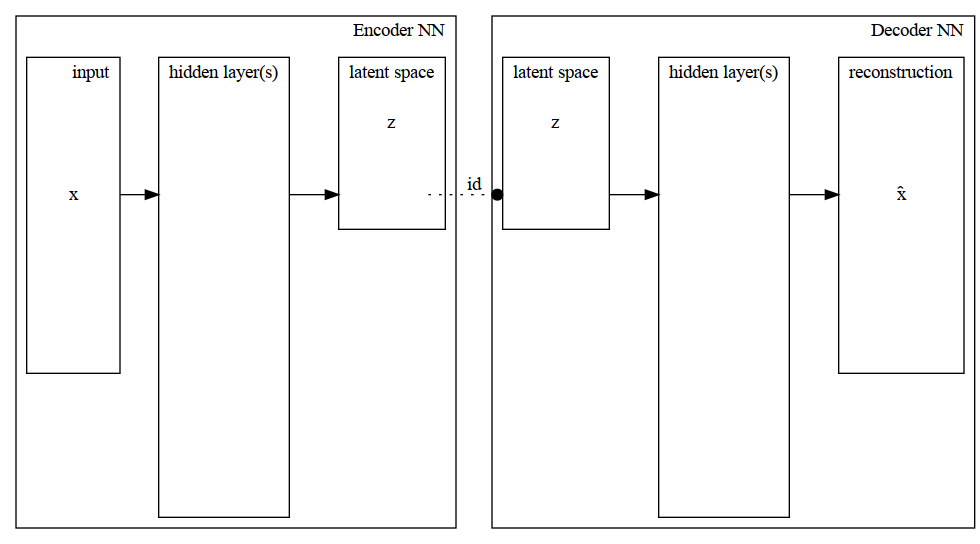
\includegraphics[width=0.9\textwidth]{./plots/autoencoderNN.gv.png}
%\label{fig:neuron1}
\caption{Autoencoder}
\label{fig:autoencoder}
%\end{framed}
\end{figure}

\end{frame}


\begin{frame}
\frametitle{Autoencoders and PCA}

(On centered data\cite{plaut2018principal})

PCA
{\small
\begin{equation}
\label{eqn:pca}
\bv{\tilde{V}} = \text{argmin}_{\W} \{
\|\X - \X \bv{W}\bv{W}^T\|_F^2 \quad : \quad \bv{W} \in \R^{n \times l}, \bv{W}^T \bv{W} =
\bv{I}_l\}
\end{equation} 
}

Linear AE
{\small
\begin{IEEEeqnarray}{C}
\label{eqn:pca2}
%\begin{aligned}
\text{argmin}_{\bv{E,D}}\{\|\X - \X \bv{E}\bv{D}\|_F^2 \quad : 
\quad \bv{E,D^T} \in \R^{n \times
l},\} \\
\label{eqn:pca3}
\bv{\tilde{W}}
\in \text{argmin}_{\W}\{\|\X - \X \bv{W}\bv{W}^{\dagger}\|_F^2 \quad : 
\quad \bv{W} \in \R^{n \times
l},\}
%\end{aligned}
\end{IEEEeqnarray}
}

$
\text{span}\{\bv{\tilde{W}}\} = \text{span}\{\bv{\tilde{V}}\}
$


\end{frame}


\begin{frame}
\frametitle{VAEs}
\begin{figure}[h]
%\begin{framed}
\centering
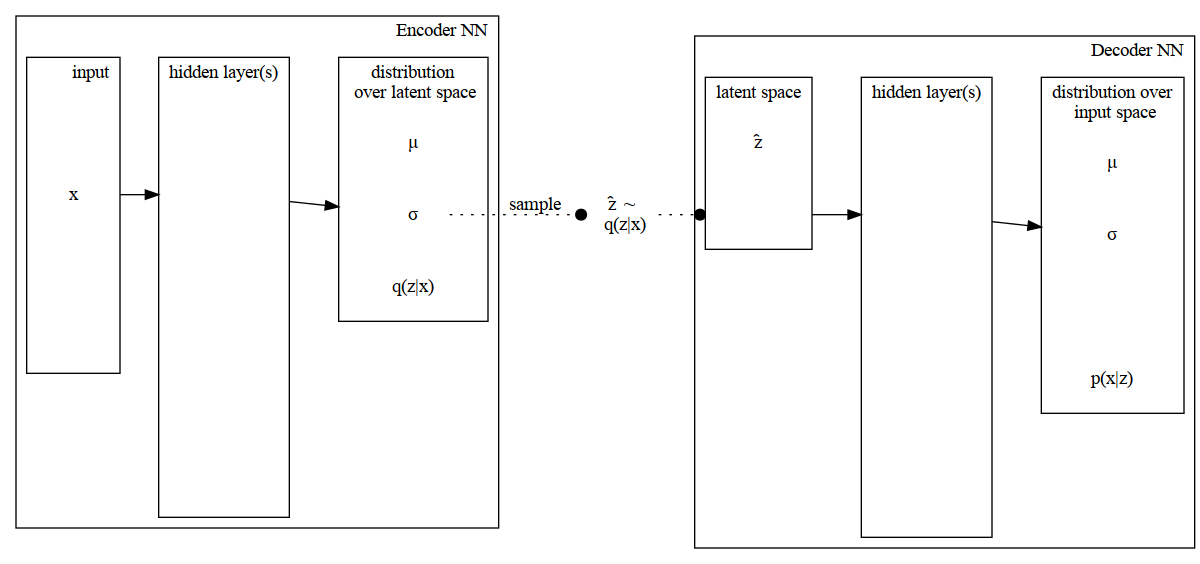
\includegraphics[width=0.99\textwidth]{./plots/vaeNN.gv.png}
%\label{fig:neuron1}
\caption{VAE}
\label{fig:vae}
%\end{framed}
\end{figure}
\end{frame}

\begin{frame}
\frametitle{VAE: encoding}
Instead of deterministic mapping, define distribution.

Define distribution on the laten space ($\z$) by mapping $x$ into the
distribution parameters e.g. $\mu(\x),\Sigma(\x)$ when we use Gaussian $q(\z|\x)
= \NN(\z |
\mu, \Sigma)$.

\end{frame}

\begin{frame}
\frametitle{VAE: decoding}
sample from the latent space $\z \sim \NN(\cdot | \mu, \Sigma)$

map $\z$ to a distribution on the input space
$p(\x | \z)$
\end{frame}

\begin{frame}
\frametitle{VAE: loss function}
The \emph{evidence lower bound (ELBO)} with respect to $p,q$ is:
\begin{IEEEeqnarray}{C}
\label{def:elbo}
-\mathcal{L}(q,p,\x) \triangleq
\int \log \frac{p(\bv{x},\bv{z})}{q(\bv{z})} d q(\bv{z}) \\
\label{def:elboX}
-\LL(q,p) \triangleq 
-\LL(q,p, \X) 
= \frac{1}{N} \sum_1^N (-\LL(q,p,\x_i) \\ 
\approx
\E_{\x} [-\LL (q,p, \x)]
\end{IEEEeqnarray}
We minimize the minus ELBO function:

\end{frame}




\begin{frame}
\frametitle{VAE: log evidence}

It can be shown that maximizing the ELBO is equivalent to 
maximinizing the "log evidence" $\log p(\X)$

{\tiny
\begin{equation}
\label{eq:elbo}
\begin{aligned}
\frac{1}{N} \log p(\bv{X}) &= \frac{1}{N} \log \int p(\bv{X},\bv{Z}) d\bv{Z} 
& \text{taking marginal} \\
& = \frac{1}{N} \log \int \frac{p(\bv{X},\bv{Z})}{q(\bv{Z})} q(\bv{Z})d\bv{Z} 
& \text{multiplying by 1 inside}\\
&=  \frac{1}{N} \log \int \frac{p(\bv{X},\bv{Z})}{q(\bv{Z})}dq(\bv{Z}) 
& \text{definition of } dq(\Z)\\
&\geq  \frac{1}{N} \int \log \frac{p(\bv{X},\bv{Z})}{q(\bv{Z})}dq(\bv{Z}) 
& \text{Jensen inequality}\\
&= \frac{1}{N} \int \sum_1^N \log \frac{p(\x_i, \z_i)}{q(\z_i)}dq(\z_i) 
& \text{using the iid property}\\
&= \frac{1}{N} \sum_1^N - \LL(q,p,\x_i)
& \text{definition of } \LL(q,p,\x_i)\\
& = -\mathcal{L}(q,p,X) \triangleq -\mathcal{L}(q,p)
& \text{again definition of } \LL(p,q) \qed
\end{aligned}
\end{equation}
}
\end{frame}

\begin{frame}
\frametitle{Monte Carlo integration}
As you can see we the loss function requires us to compute an integral, which
usually cannot be done analytically.

Instead the integral is approximated by Monte Carlo integration.

{\small
\begin{equation}
\begin{aligned}
\text{sample  } \z_i \sim q(\z | \x) \text{   then :}\\
\LL(p,q,\x) = 
\int - \log \frac{p(\x|\z)p(\z)}{q(\z|\x)}dq(\z|\x) \\
= \int -\log p(\x|\z)dq(\z|\x) + 
\int \log \frac{q(\z|\x)}{p(\z)}dq(\z|\x) \\
\approx \frac{1}{k} \sum_{i=1}^k [-\log p(\x|\z_i)
+ \log \frac{q(\z_i|\x)}{p(\z_i)} ]
\label{eq:elbomc}
\end{aligned}
\end{equation}
}

\end{frame}


\begin{frame}
\frametitle{VAE: compounding the latent distribution}
More complicated distributions such as mixture distribution
can be modelled by "unpacking" the latent $\z$ and the observed $\x$
%into several random variables, each with different type of distribution.
%We can describe a more complex distribution by unpacking them and describe the
%dependencies between them.
%This is done in the following way:
\label{VAE-specs}
\begin{enumerate}
\item{} Define the set of observed random vectors $\x_1, \x_2, \dots \x_k$, and 
the set of latent random vectors and stochastic parameters $\z_1, \dots \z_l$.
\item{} Specify how to factor the generative model $p(\x_1,\dots, \x_k| \z_1
\dots , \z_l)$
\item{} Specify how to factor the inference model $q(\z_1 \dots \z_l | \x1,
\dots \x_k)$
\item{} Choose appropriate priors $p(\z_i)$ and
\item{} Choose appropriate distribution families for the $\x_i$ and $\z_i$,
and choose priors $p(\z_i)$.
\end{enumerate}

%This is easiest to show graphically.
\end{frame}

\begin{frame}
\frametitle{VAE: Graphical representation}
Evry distribution can be represented by a DAG. Nodes represent random variables
(and also priors), and directed arrows represent conditional dependency.

\end{frame}


\begin{frame}
\frametitle{VAE: base case}

\begin{figure}[h]
%\begin{framed}
\centering
\begin{subfigure}[b]{0.2\textwidth}
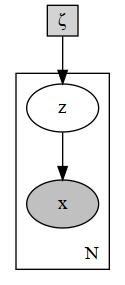
\includegraphics[width=\textwidth]{plots/vae_p.gv.png}
\caption{generative model $p(x,z)$}
\end{subfigure}
\begin{subfigure}[b]{0.2\textwidth}
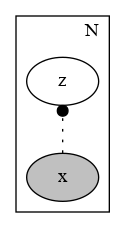
\includegraphics[width=\textwidth]{plots/vae_q.gv.png}
\caption{inference model $q(z|x)$}
\end{subfigure}
\begin{subfigure}[b]{0.2\textwidth}
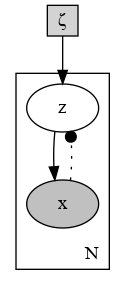
\includegraphics[width=\textwidth]{plots/vae.gv.png}
\caption{the combined graphical model}
\end{subfigure}
\caption{VAE graphical model}
\label{fig:vae_model}
%\end{framed}
\end{figure}

\end{frame}

\begin{frame}
\frametitle{VAE: patholocigacl case}

\begin{figure}[h]
\centering
\begin{subfigure}[b]{0.2\textwidth}
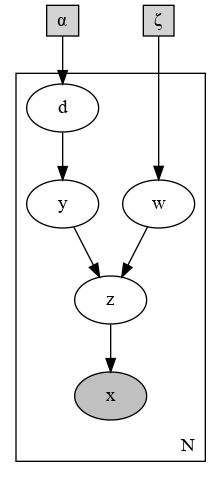
\includegraphics[width=\textwidth]{plots/dirichlet_gmm_p.gv.png}
\caption{generative model $p(x,z)$}
\end{subfigure}
\begin{subfigure}[b]{0.2\textwidth}
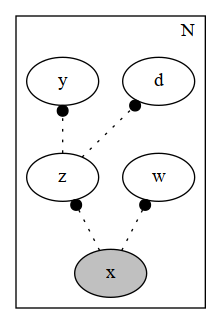
\includegraphics[width=\textwidth]{plots/dirichlet_gmm_q.gv.png}
\caption{inference model $q(z|x)$}
\end{subfigure}
\begin{subfigure}[b]{0.4\textwidth}
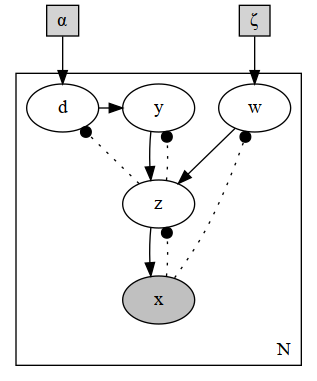
\includegraphics[width=\textwidth]{plots/dirichlet_gmm.gv.png}
\caption{the combined graphical model}
\end{subfigure}
\caption{\gmvae graphical model}
\label{fig:gmvae_model}
\end{figure}


\end{frame}

\begin{frame}
\frametitle{\gmvae generative model}

\begin{columns}[T]
%\begin{column}{5cm}
\begin{column}{0.5\linewidth}
\begin{figure}[h]
\centering
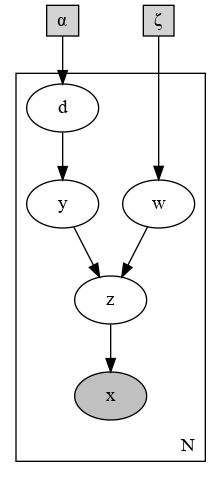
\includegraphics[width=0.4\textwidth]{plots/dirichlet_gmm_p.gv.png}
%\caption{\gmvae: generative model}
\end{figure}
\end{column}

%\begin{column}{5cm}
\begin{column}{0.5\linewidth}
{\tiny
\begin{equation}
\label{eq:gmmfact}
\begin{aligned}
&p(\x, \y, \z, \w, \dd) &=\quad& 
p(\x | \z) p(\z | \w, \y) p(\y | \dd) p(\dd) p(\w) \\
&p(\w) &=\quad& \NN(\w | \bv{0},\bv{1}) \\
&p(\dd) &=\quad& \text{Dir}(\dd | \alpha) \\
&p(\y | \dd) &=\quad& \text{Cat}(\y | \dd) \\
&p(\z | \w, \y) &=\quad& \NN(\z | \mu(\w)_{\y}, \sigma(\w)_{\y})) \\
&p(\x | \z) &=\quad& \NN(\x | \mu(\z), \sigma(\z))
\end{aligned}
\end{equation}
}
\end{column}
\end{columns}
\end{frame}

\begin{frame}
\frametitle{\gmvae inference model}
\begin{columns}[T]
\begin{column}{0.5\linewidth}
\begin{figure}[h]
\centering
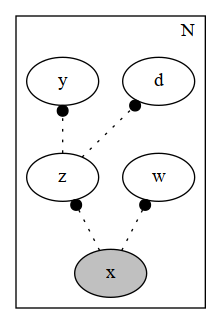
\includegraphics[width=0.4\textwidth]{plots/dirichlet_gmm_q.gv.png}
%\caption{\gmvae: generative model}
\end{figure}
\end{column}

\begin{column}{0.5\linewidth}
{\tiny
\begin{equation}
\label{eq:gmmqfact}
\begin{aligned}
&q(\y, \z, \w, \dd | \x) &=& 
&q(\z | \x) q(\w | \x) q(\y | \z) q(\dd | \z) \\
&q(\z | \x) &=& &\NN(\z | \mu_z(\x), \sigma_z(\x)) \\
&q(\w | \x) &=& &\NN(\w | \mu_w(\x), \sigma_w(\x)) \\
&q(\y | \z) &=& &\text{Cat}(\y | f(\z)) \\
&q(\dd | \z) &=& &\text{Dir}(\dd | g(\z))
\end{aligned}
\end{equation}
}
\end{column}
\end{columns}
\end{frame}


\begin{frame}
\frametitle{\gmvae loss function}
The loss function remains the -ELBO and we can break it into
different terms:

{\tiny
\begin{IEEEeqnarray}{lC}
\LL(p,q,\x) &= 
\int - \log \frac{p(\x,\y,\z,\w,\dd)}{q(\z,\y,\w,\dd | \x)} dq(\z,\y,\w,\dd |
\x) \\ 
&= \int - \log 
\frac{p(\x | \z) p(\z | \w, \y) p(\y | \dd) p(\w) p(\dd)}
{q(\z | \x) q(\w | \x) q(\y | \z) q(\dd | \z)} dq \\
&= \int - \log p(\x | \z) dq \\
\label{dgmmrecloss}
&+ \int \log \frac{q(\z | \x)}{p(\z | \w, \y)}dq \\
\label{dgmmzloss}
&+ \int \log \frac{q(\w | \x)}{p(\w)}dq \\
\label{dgmmwloss}
&+ \int \log \frac{q(\y | \z)}{p(\y | \dd)}dq \\
\label{dgmmyloss}
&+ \int \log \frac{q(\dd | \z)}{p(\dd)}dq
\label{dgmmdloss}
\end{IEEEeqnarray}
}
\end{frame}

\begin{frame}
\frametitle{\gmvae: supervised case}

\begin{figure}[h]
%\begin{framed}
\centering
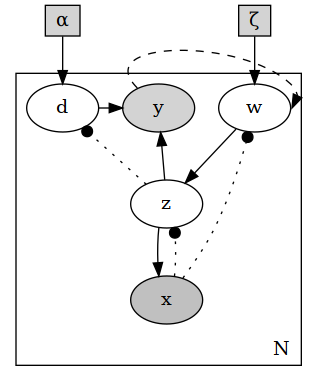
\includegraphics[width=0.5\textwidth]{plots/dirichlet_gmm_supervised.gv.png}
\caption{\gmvae: the supervised case, where $\y$ is an observed variable.
}
\label{fig:dirgmm_sup}
%\end{framed}
\end{figure}

\end{frame}

\begin{frame}
\frametitle{the conditional flavor of \gmvae}
\begin{figure}[h]
\centering
\begin{subfigure}[b]{0.45\textwidth}
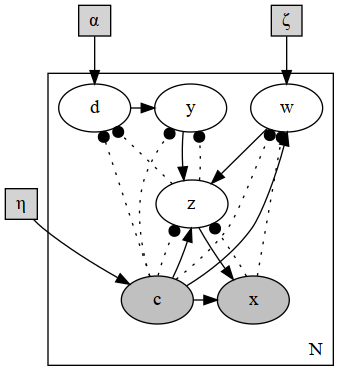
\includegraphics[width=0.99\textwidth]{plots/dirichlet_gmm_cvae.v2.gv.png}
\caption{\gmvae (cond.), unsupervised case. Sorry for the arrow clutter}
\label{fig:dirgmmcvae}
\end{subfigure}
\begin{subfigure}[b]{0.45\textwidth}
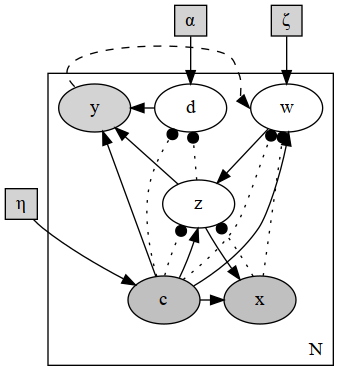
\includegraphics[width=0.99\textwidth]{plots/dirichlet_gmm_cvae_supervised.v2.gv.png}
\caption{\gmvae (cond.), supervised case}
\label{fig:dirgmmcvae_super}
\end{subfigure}
\end{figure}
\end{frame}

\begin{frame}
\frametitle{Tests on MNIST}
\begin{figure}[h]
%\begin{framed}
\centering
\begin{subfigure}[b]{0.80\textwidth}
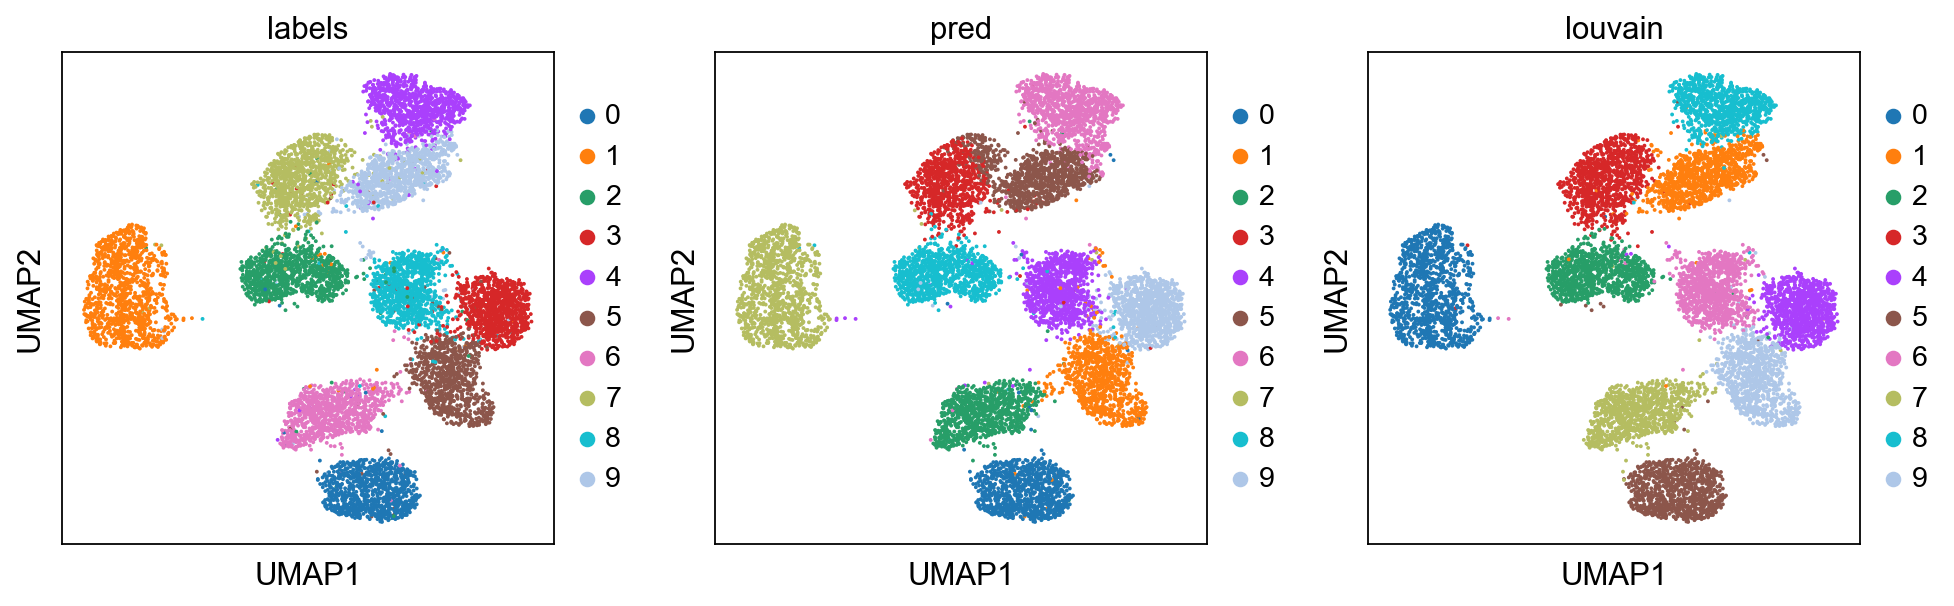
\includegraphics[width=\textwidth]{images/gmmvae_mnist_us_latent_umap.png}
\caption{UMAP of the latent space}
\label{fig:mnist_us_latent}
\end{subfigure}
\begin{subfigure}[b]{0.3\textwidth}
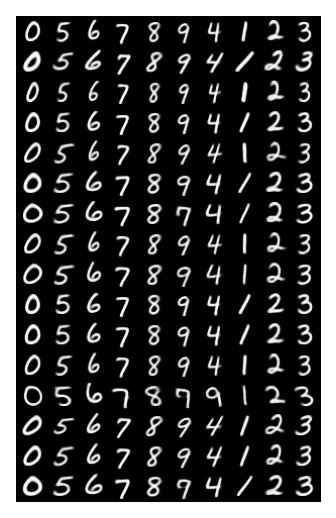
\includegraphics[width=\textwidth]{images/gmmvae_mnist_us_samples2.png}
\caption{Randomly generated samples}
\label{fig:mnist_us_samples}
\end{subfigure}
\caption{\gmvae: unsupervised learning of MNIST. This particular model
achieved 0.93 accuracy which probably could be a little bit further
improved with fine-tune training. The Louvain clustering of the latent space is even better
than the prediction.}
\label{fig:mnist_us_10}
%\end{framed}
\end{figure}

\end{frame}

\begin{frame}
\frametitle{Testing on synthetic conditional-categorical "blobs" dataset}
\begin{figure}[h]
\centering
\includesvg [width=0.9\textwidth]{images/blobs3d_pca.svg}
\caption{The toy dataset, showing a 3d plot of its 3 major PCA components.
}
\label{fig:blobs_3d}
\end{figure}
\end{frame}


\begin{frame}
\frametitle{$\w$ embeding}
\begin{figure}[h]
\centering
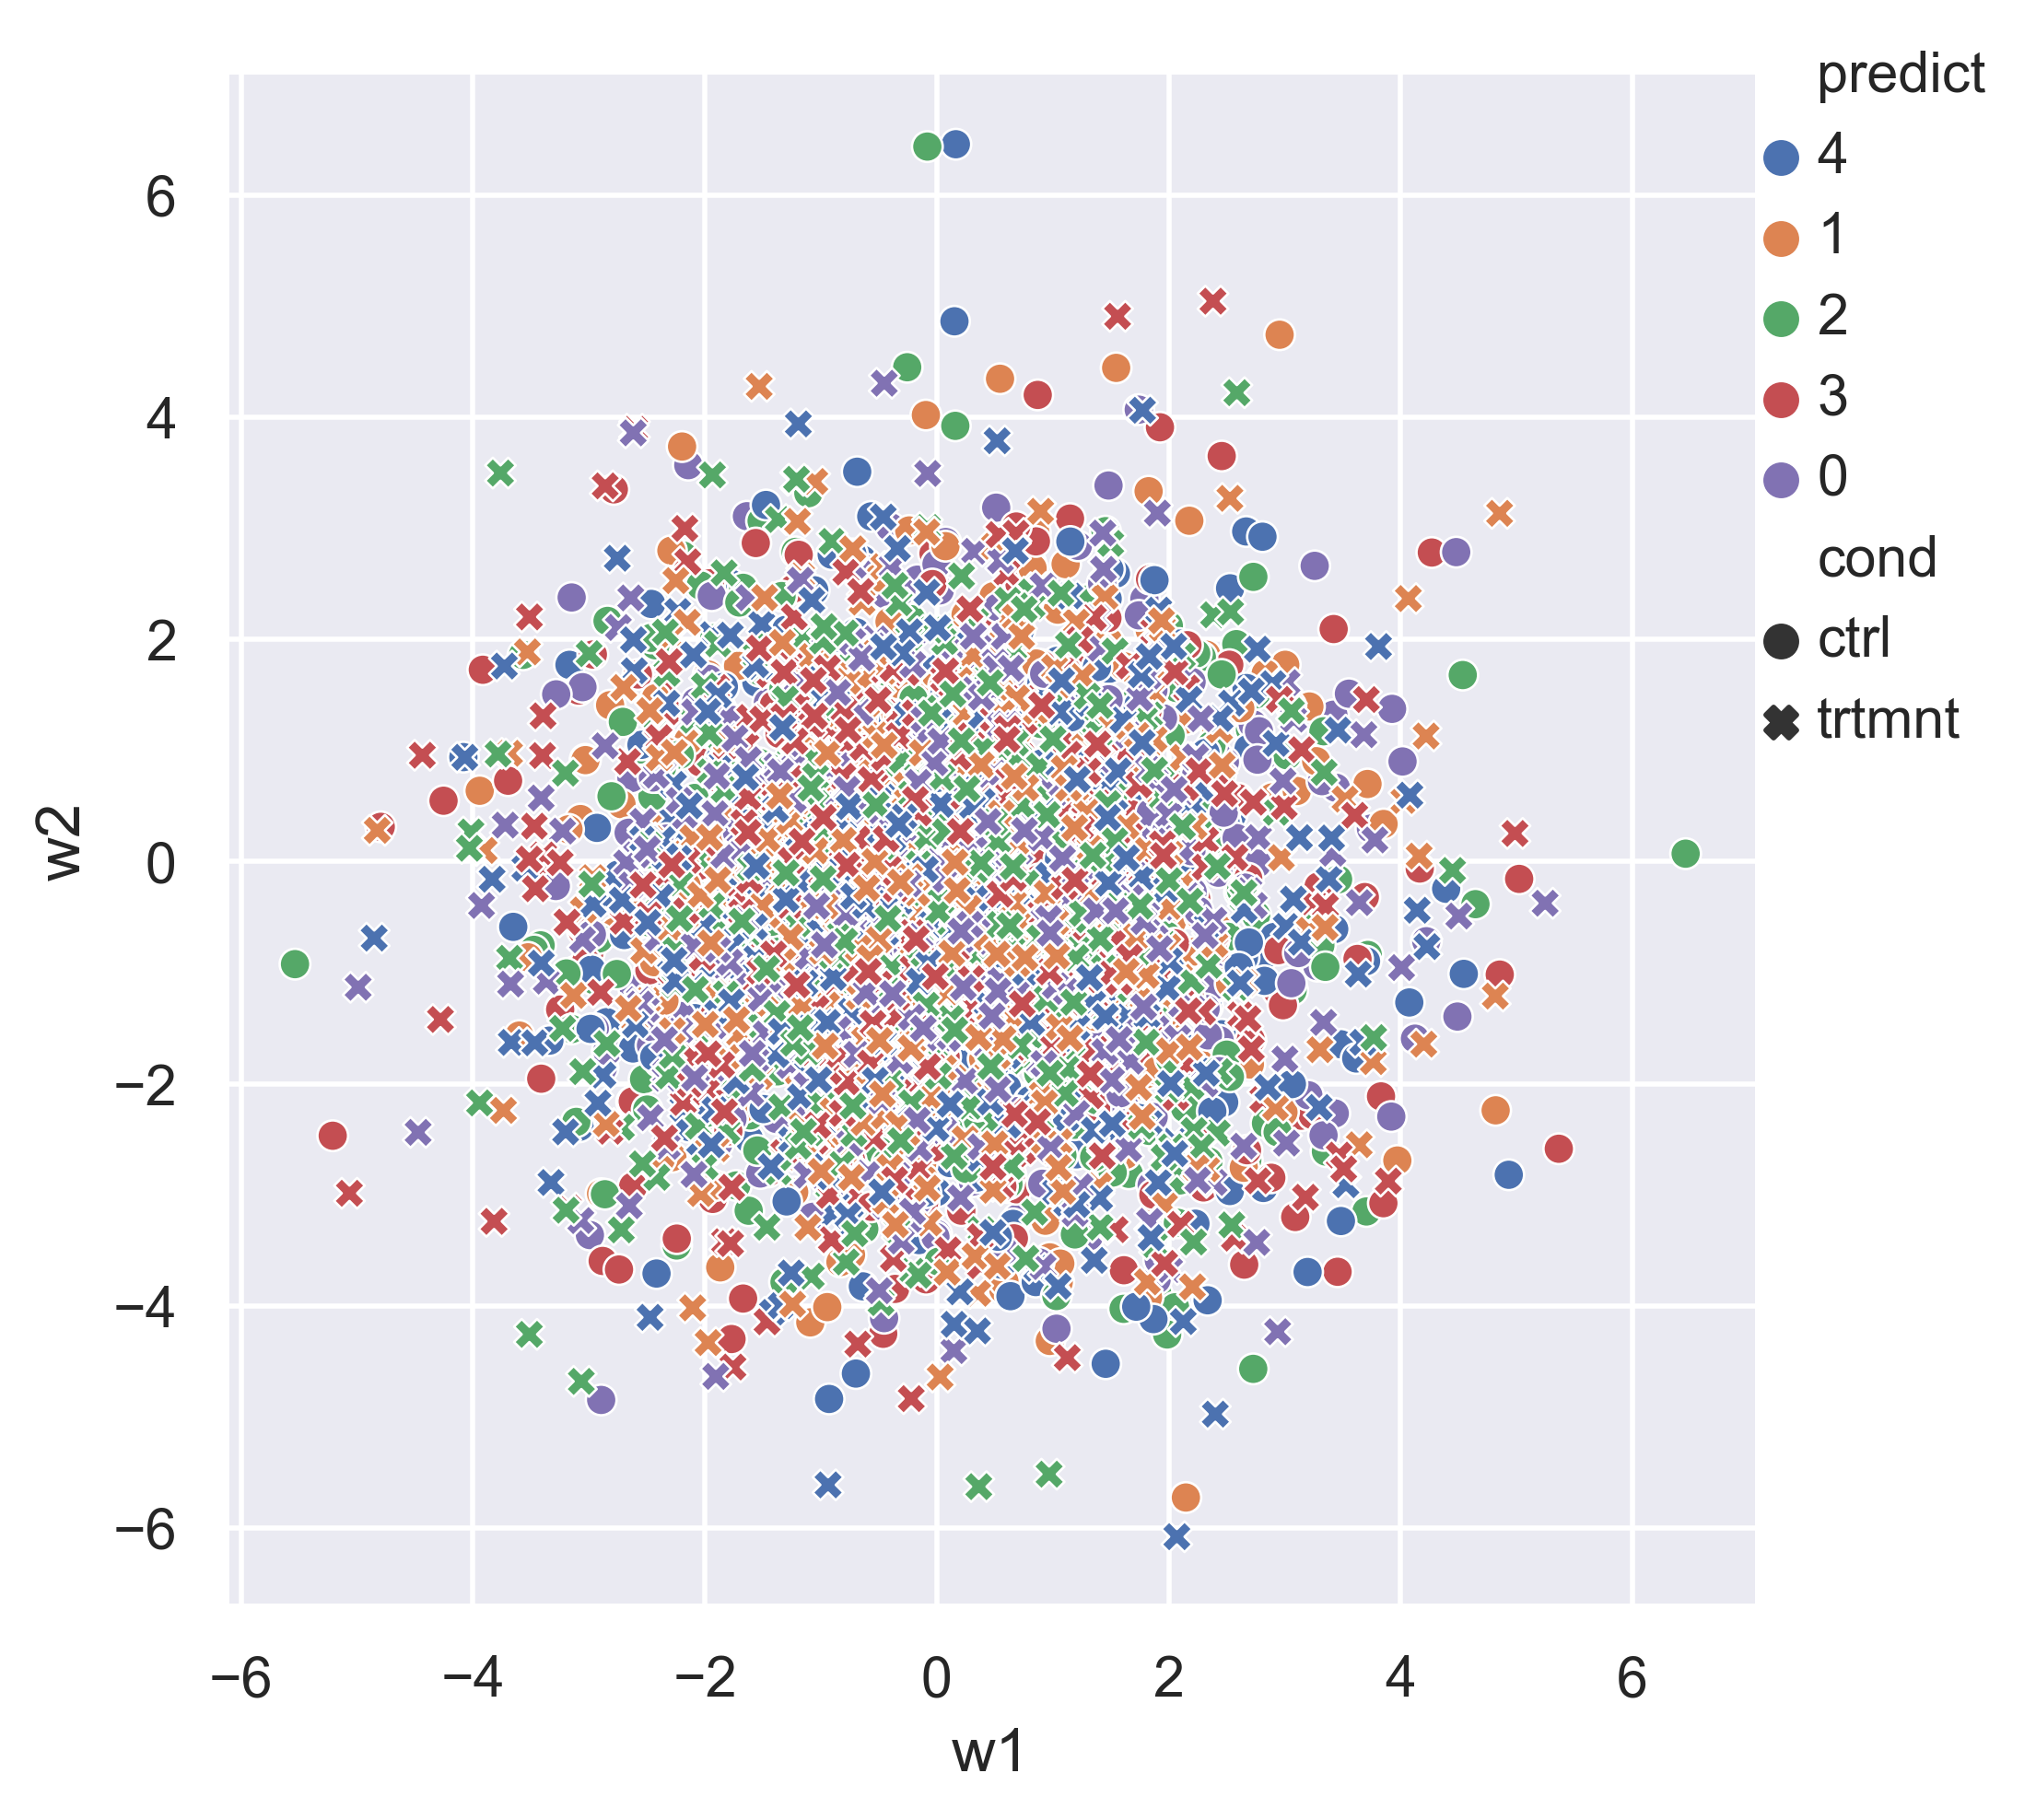
\includegraphics[width=0.8\textwidth]{images/blobs_cgmvae_learnedprior_w.png}
\caption{Random sampling from the encoded distribution of the $\w$ space. 
}
\label{fig:blobs_lp_w}
\end{figure}
\end{frame}


\begin{frame}
\frametitle{$\z$ embeding}
\begin{figure}[h]
\centering
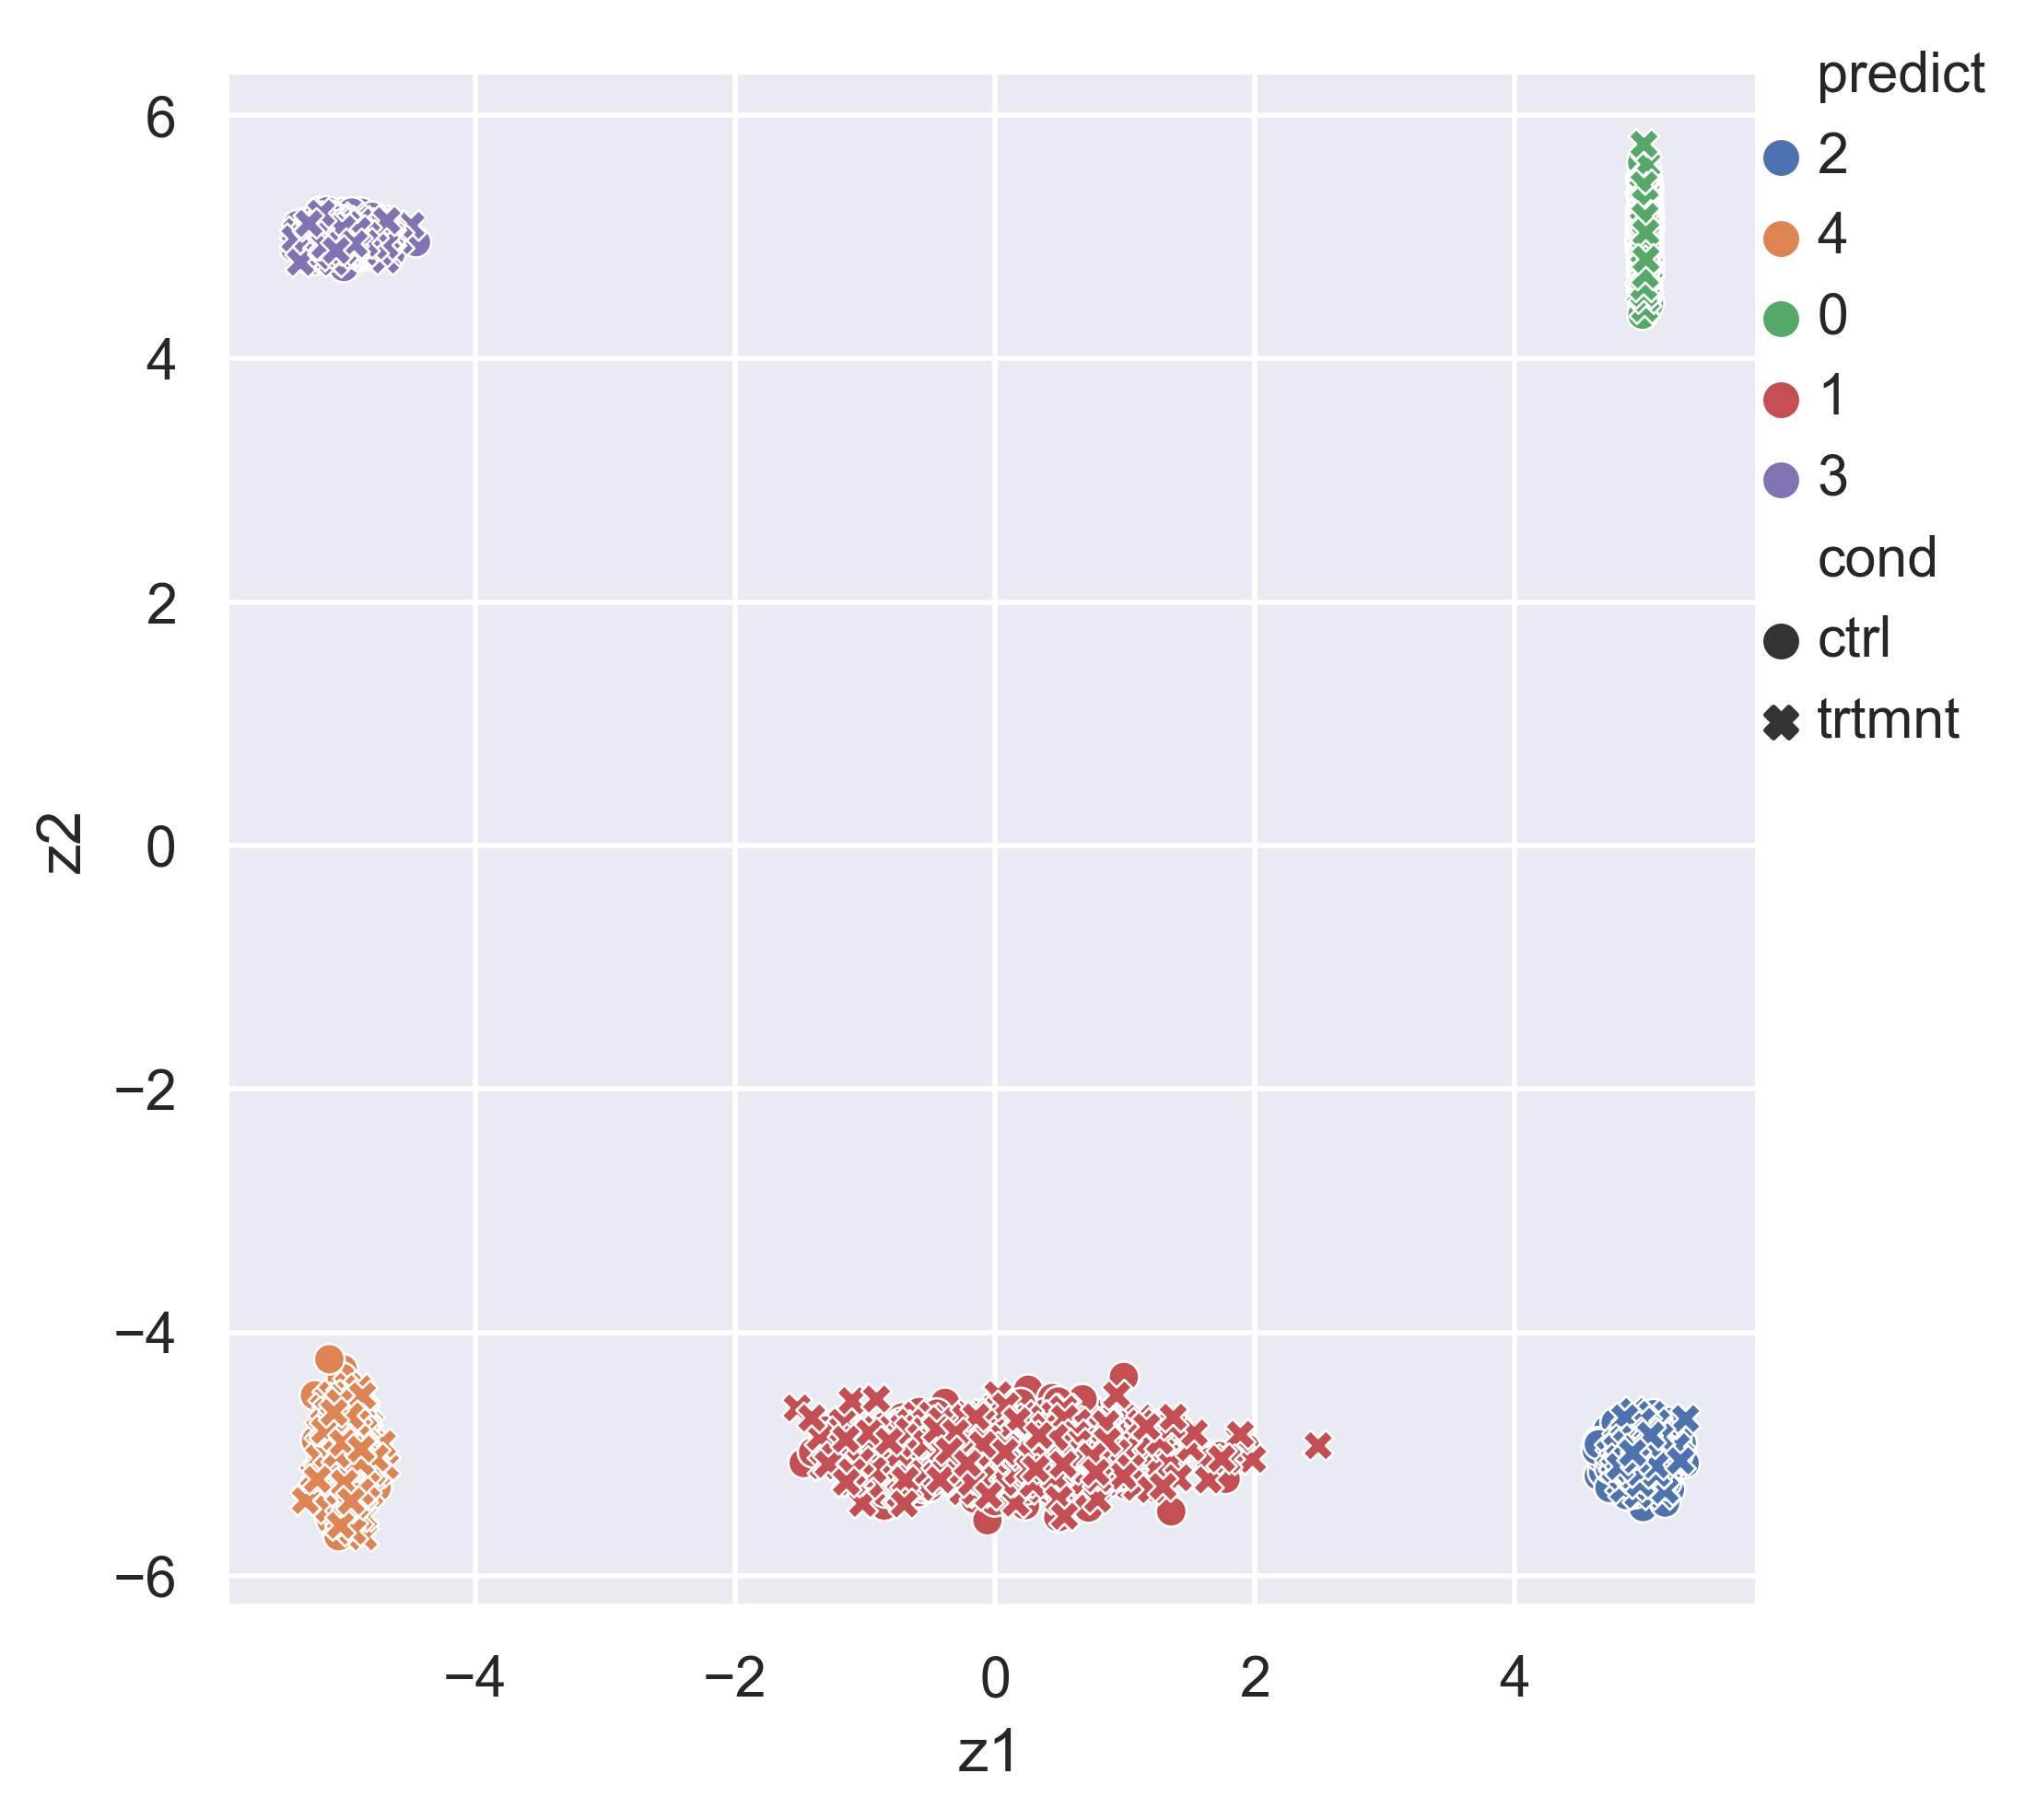
\includegraphics[width=0.8\textwidth]{images/blobs_cgmvae_stdprior_z.png}
\caption{Sampling from encoded $\z$ space, fixed standard normal prior case.
}
\label{fig:blobs_nop_z}
\end{figure}
\end{frame}

\begin{frame}
\frametitle{Transfer learning}
\begin{figure}[h]
\centering
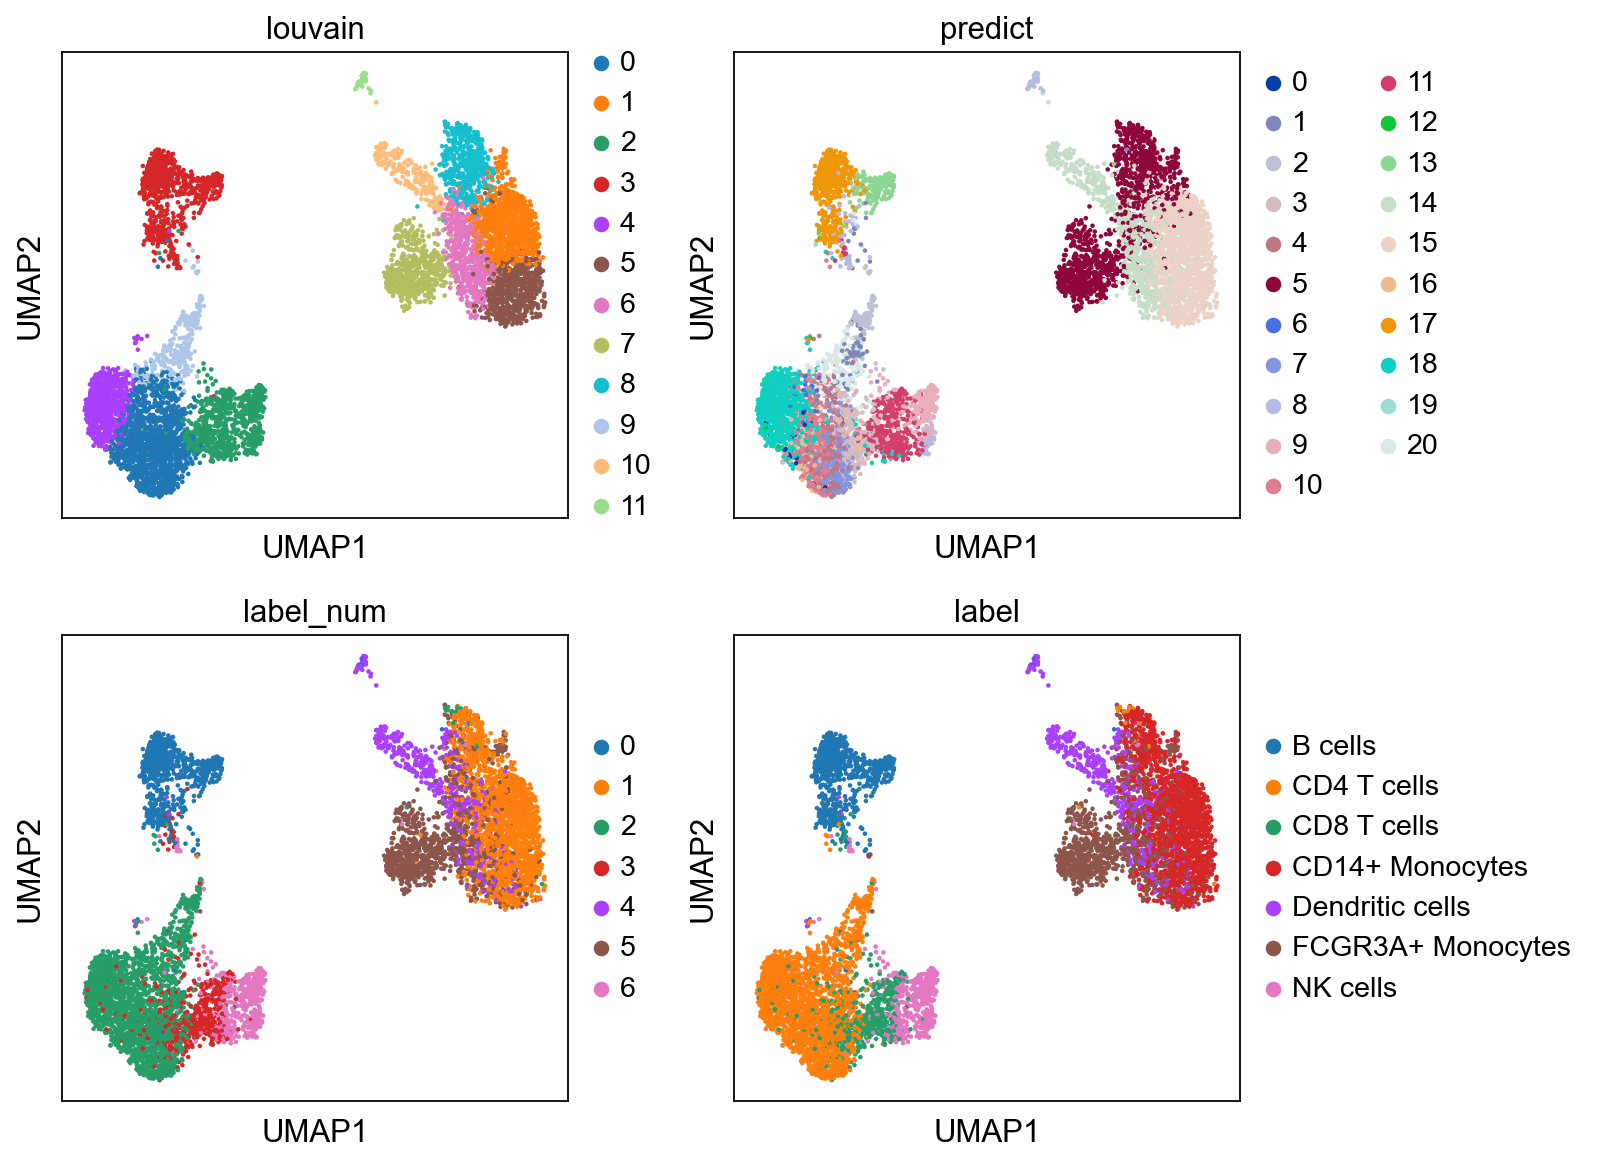
\includegraphics[width=0.8\textwidth]{images/gmmvae_Kang_control_train_us_21c_umap.png}
\caption{
UMAP of PCA space of the Kang train data. 
}
\label{fig:kang_control_train_gmvae_us_umap}
\end{figure}
\end{frame}

\begin{frame}
\frametitle{Transfer learning}
\begin{figure}[h]
\centering
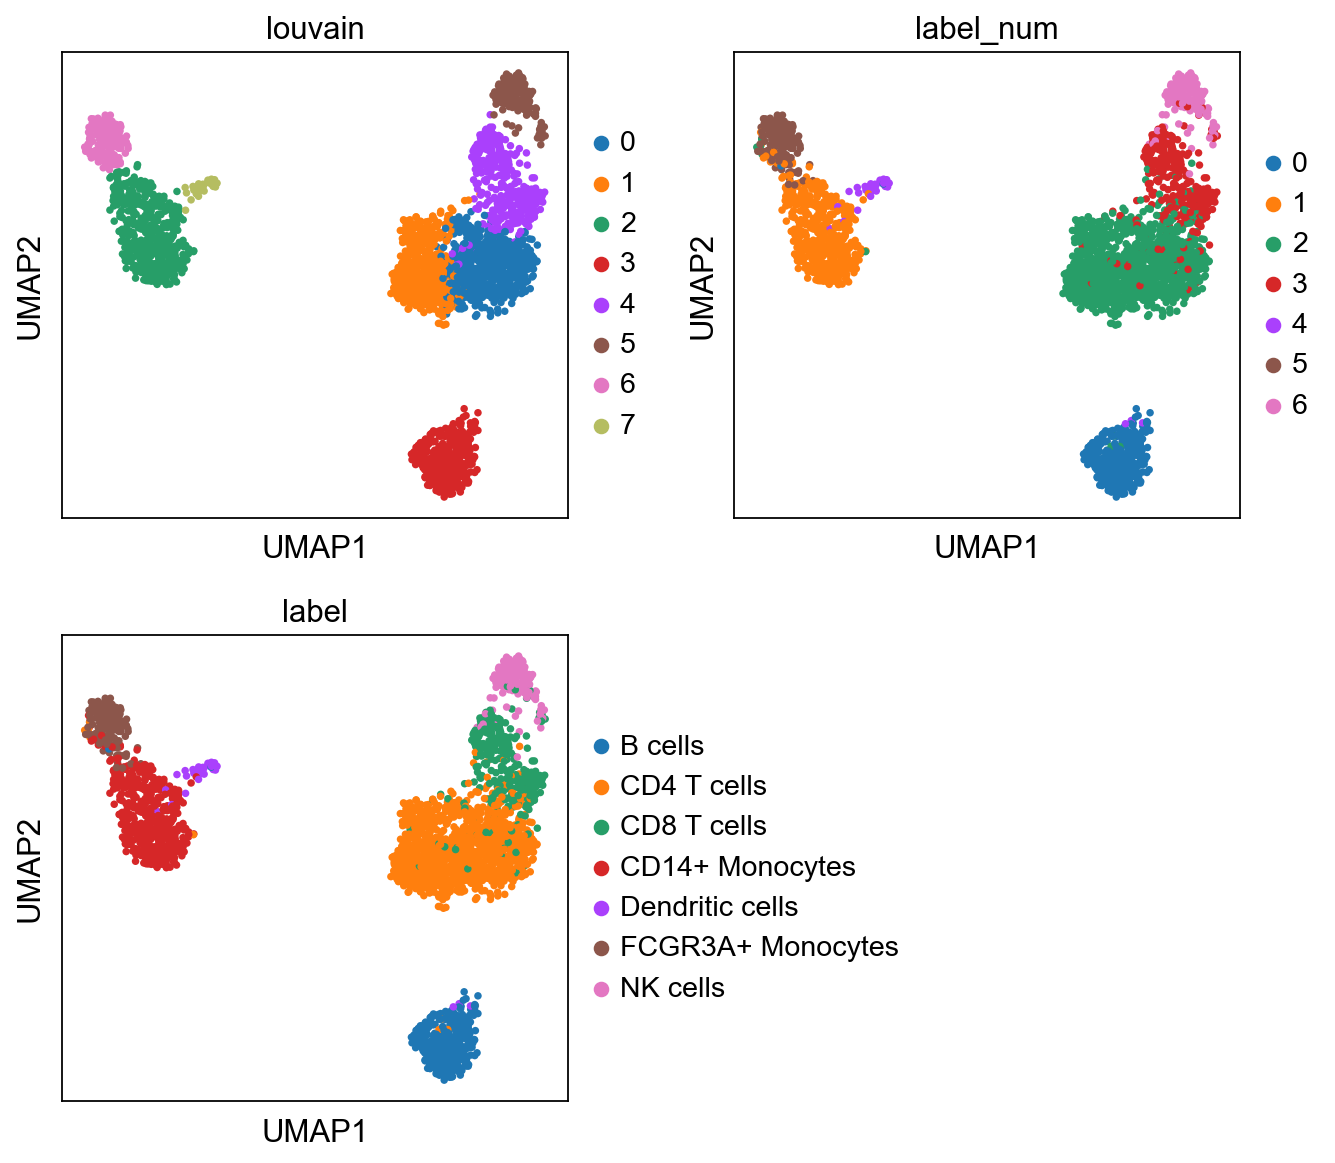
\includegraphics[width=0.8\textwidth]{images/gmmvae_zheng_new_louvain_umap1.png}
\caption{
UMAP of the Zheng dataset.
}
\label{fig:zheng_pca_umap_new}
\end{figure}

\end{frame}


\begin{frame}
\frametitle{Transfer learning}
\begin{figure}[h]
\centering
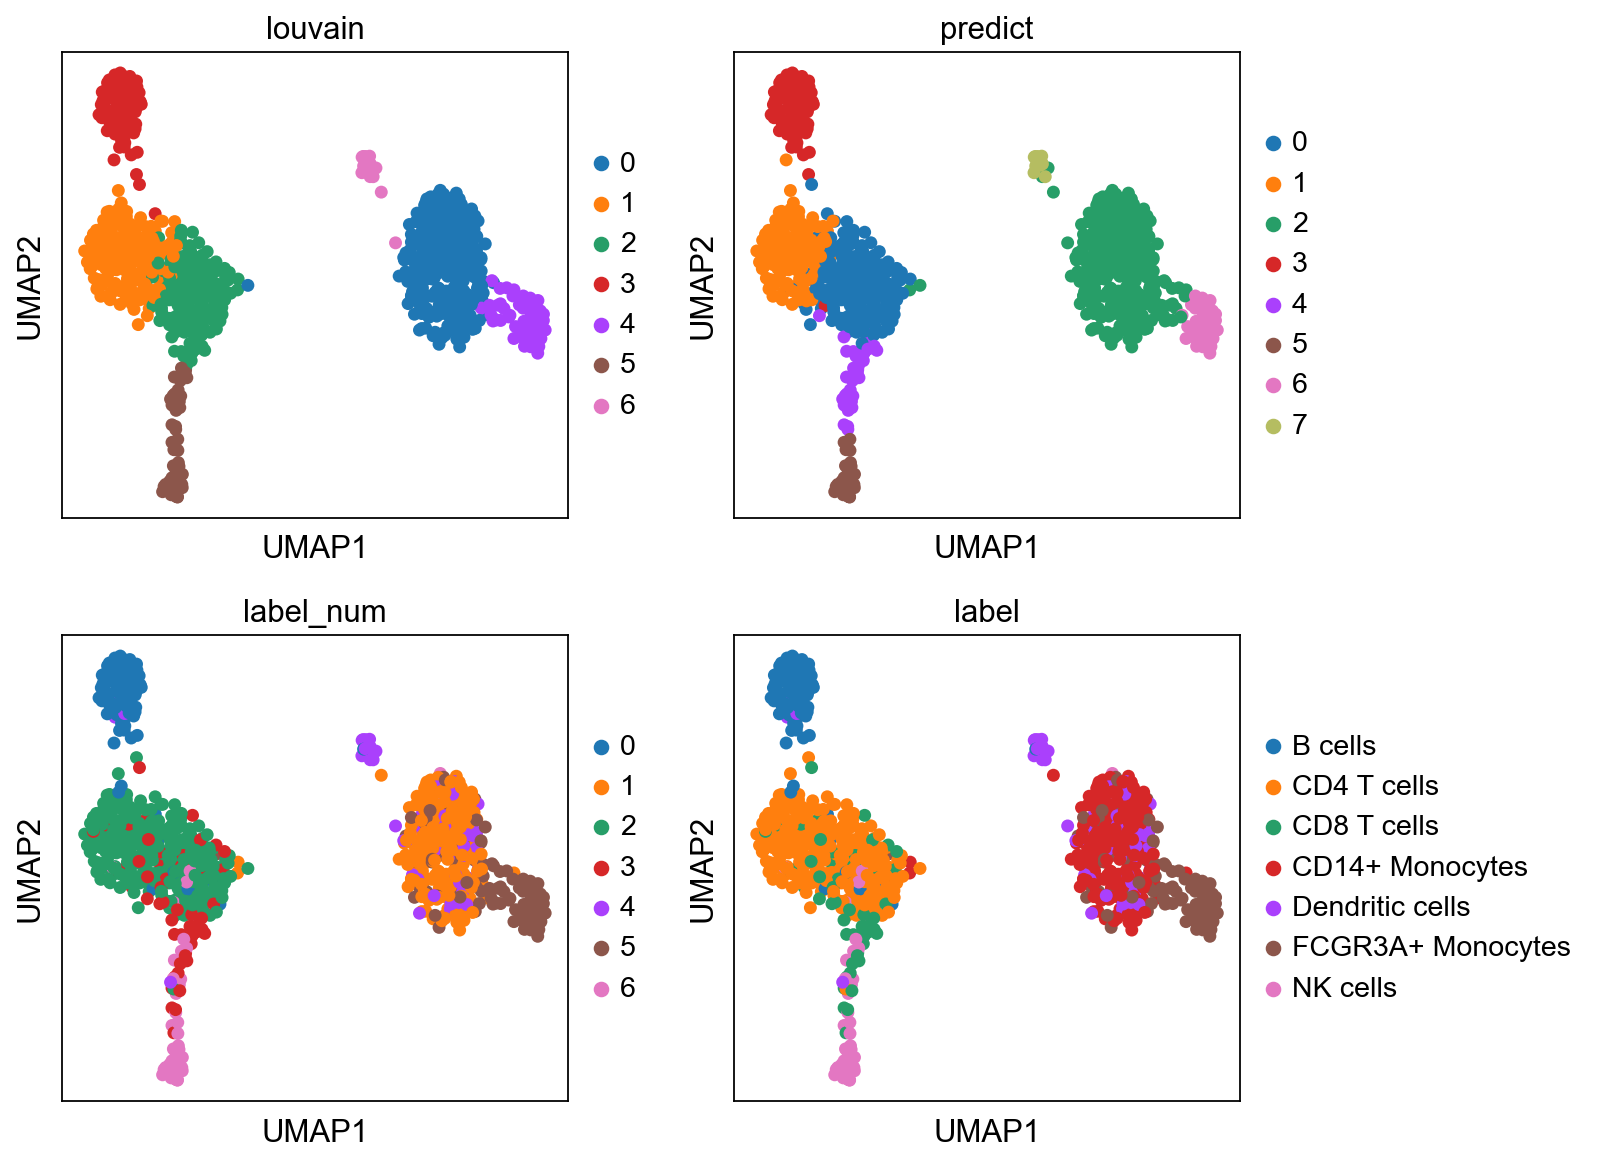
\includegraphics[width=0.7\textwidth]{images/gmmvae_kang_new_latent_louvain_pred_umap1.png}
\caption{
UMAP of the latent space of the Kang validation subset (the holdout).
}
\label{fig:kang_new_latent}
\end{figure}
\end{frame}

\begin{frame}
\frametitle{converting treatment effect}
\begin{figure}[h]
\centering
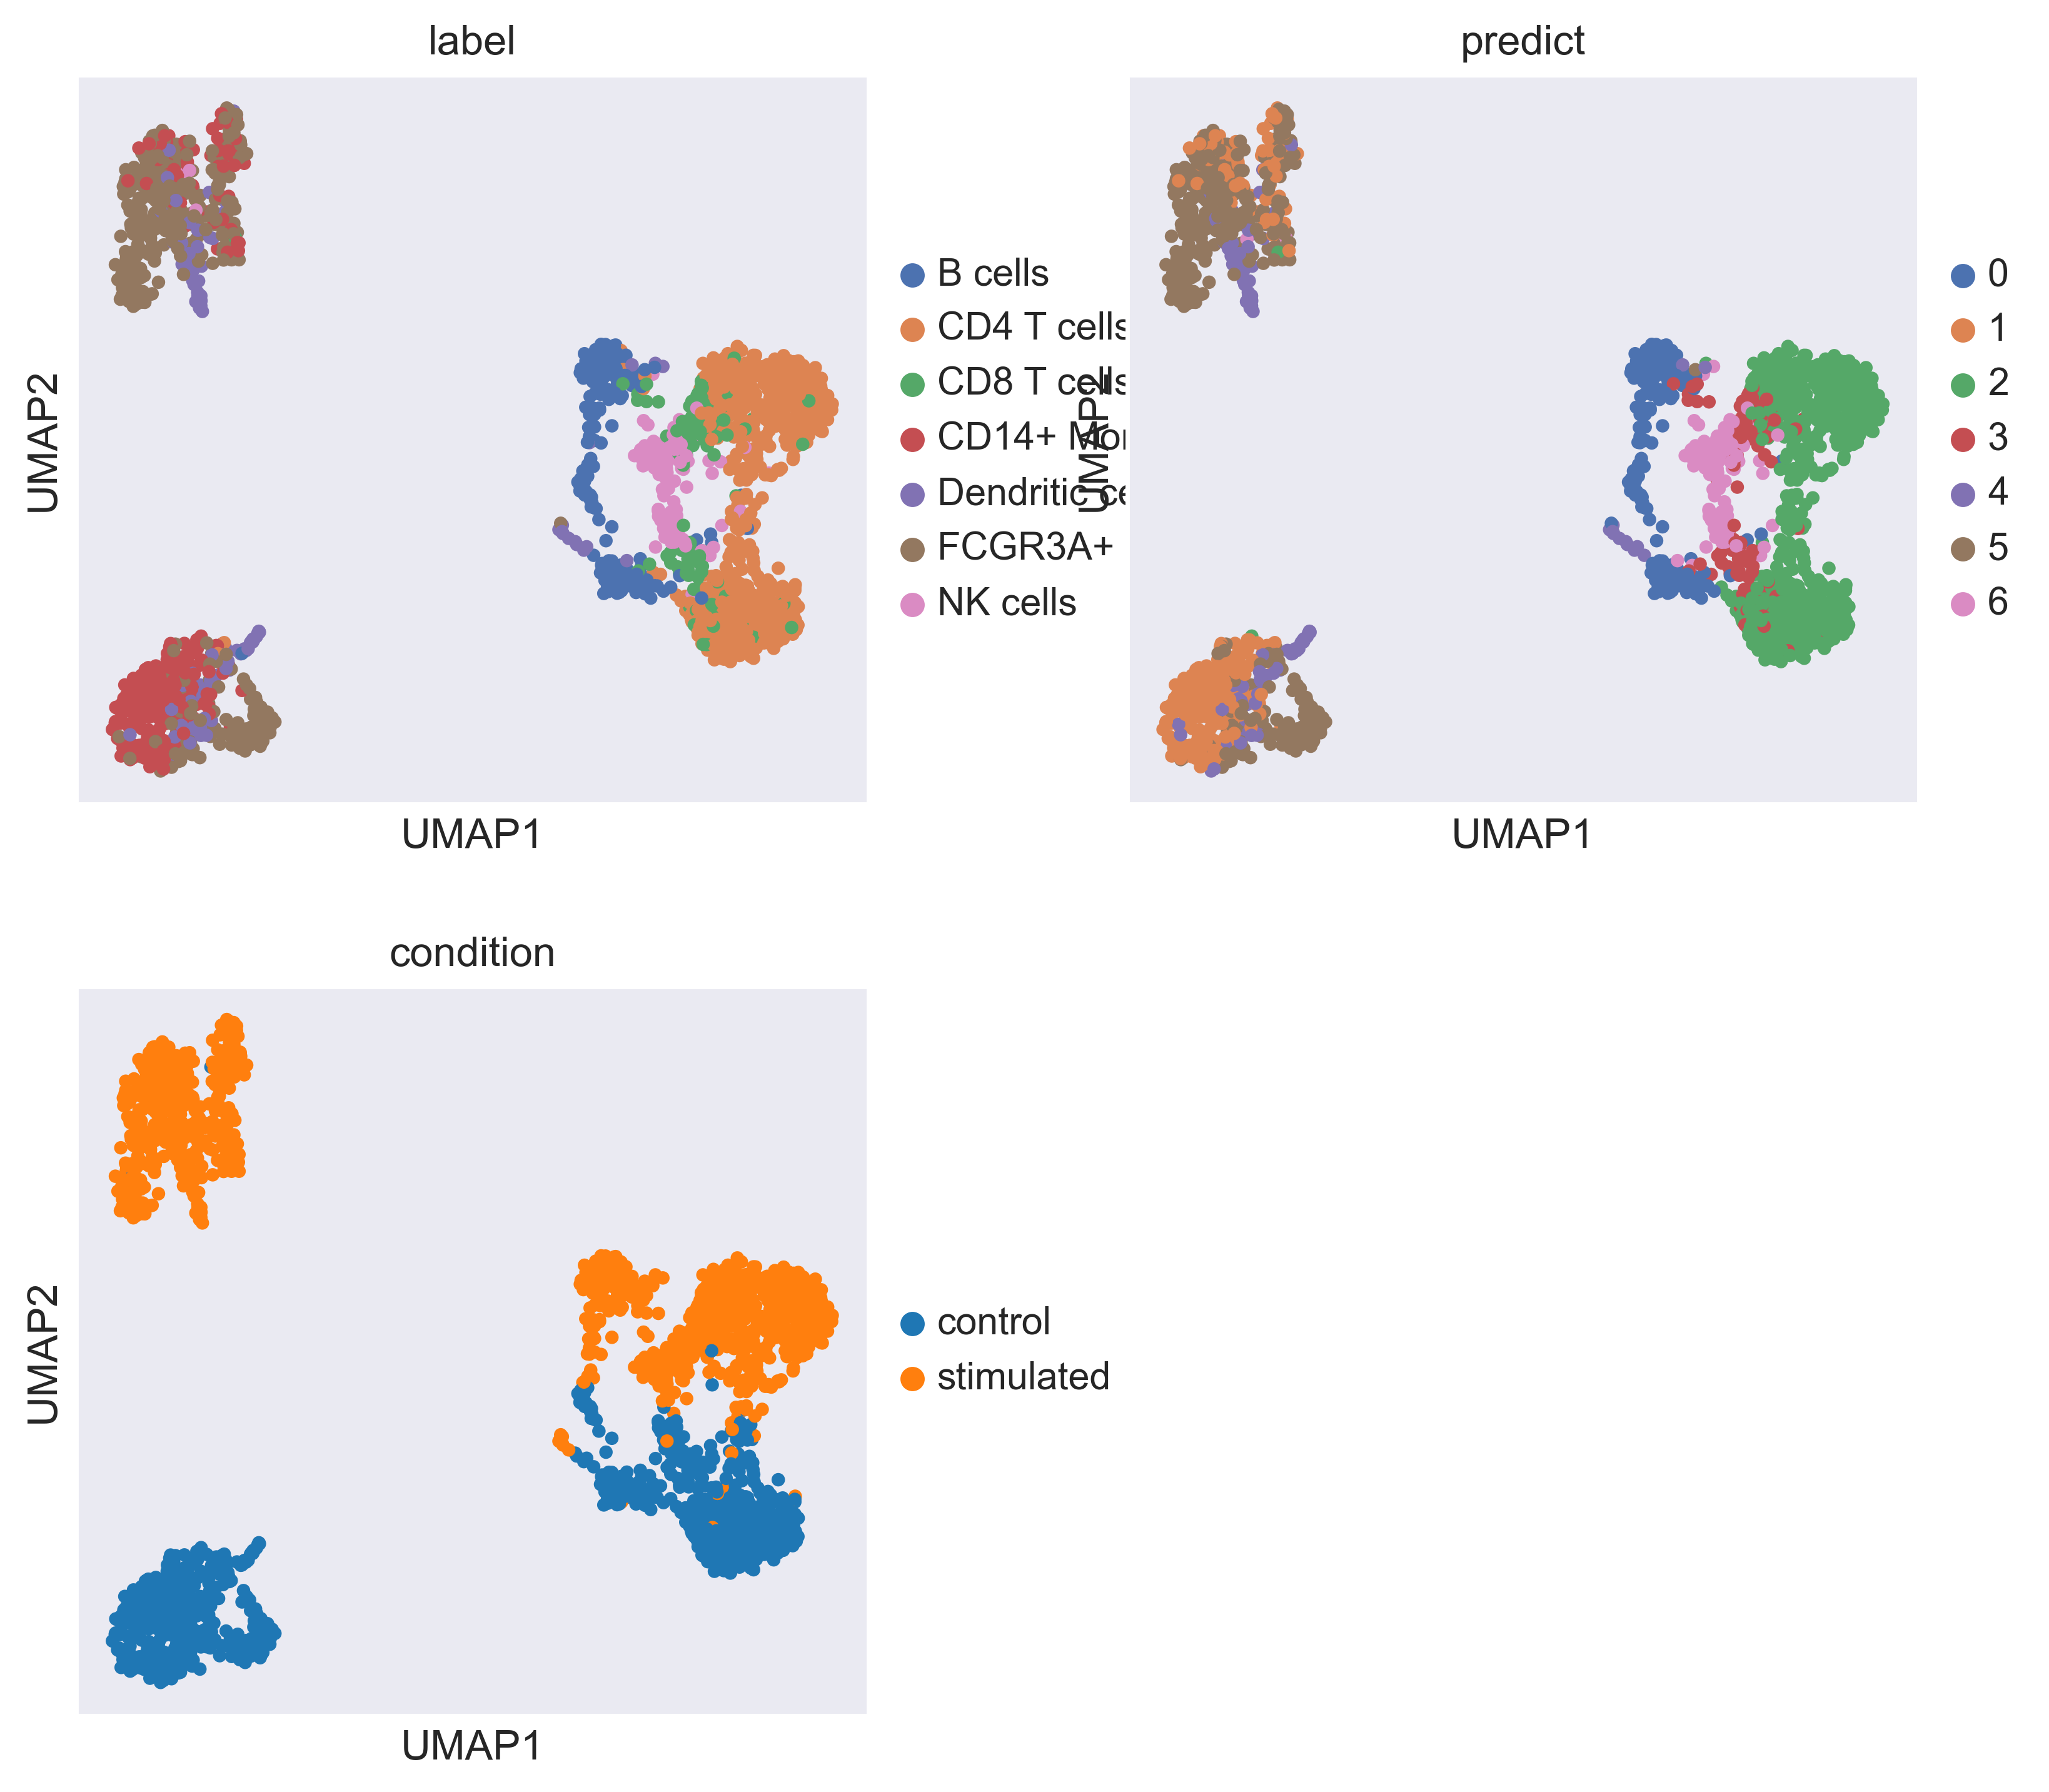
\includegraphics[width=0.8\textwidth]{images/Kang_super_val_umap.png}
\caption{UMAP of the Kang validation dataset
}
\label{fig:Kang_super_val_umap}
\end{figure}
\end{frame}

\begin{frame}
\frametitle{converting treatment effect}
\begin{figure}[h]
\centering
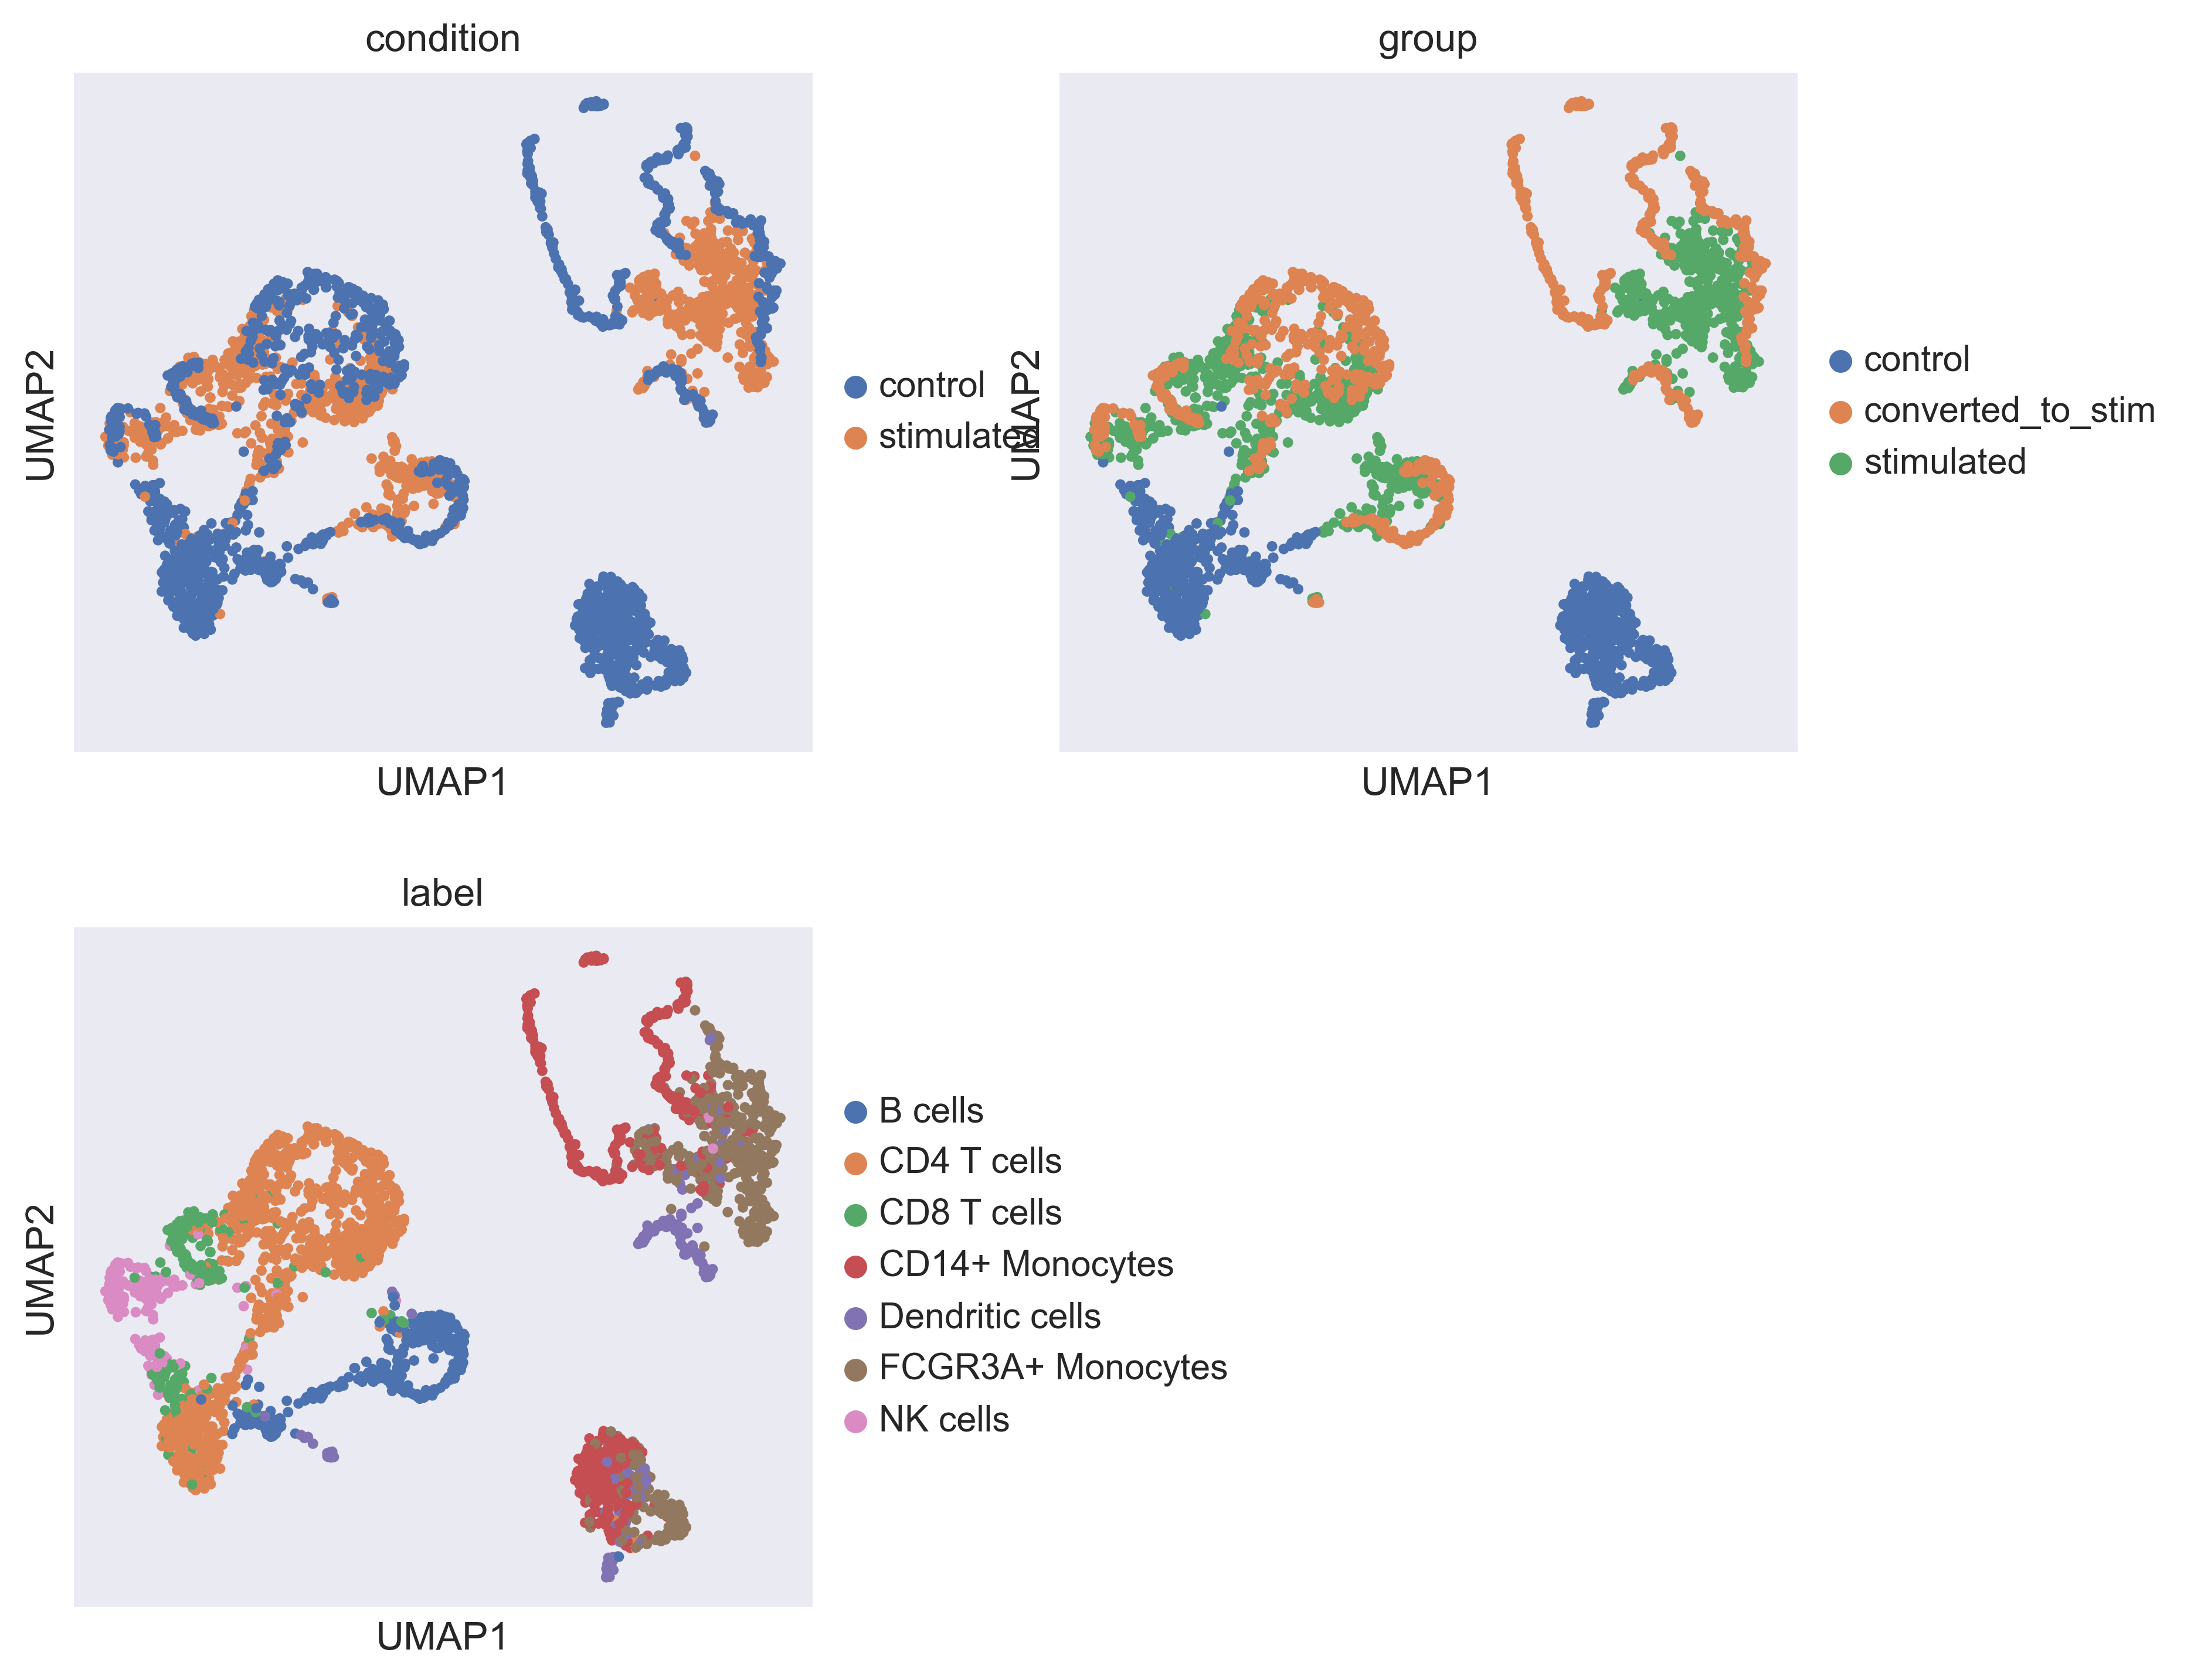
\includegraphics[width=0.8\textwidth]{images/Kang_super_val_umap_converted_control.png}
\caption{
UMAP of the combined validation subset with its control group remapped into
stimulated state.
}
\label{fig:Kang_super_val_umap_converted_control}
\end{figure}
\end{frame}

\begin{frame}
\frametitle{converting treatment effect}
\begin{figure}[h]
\centering
\begin{subfigure}[b]{0.49\textwidth}
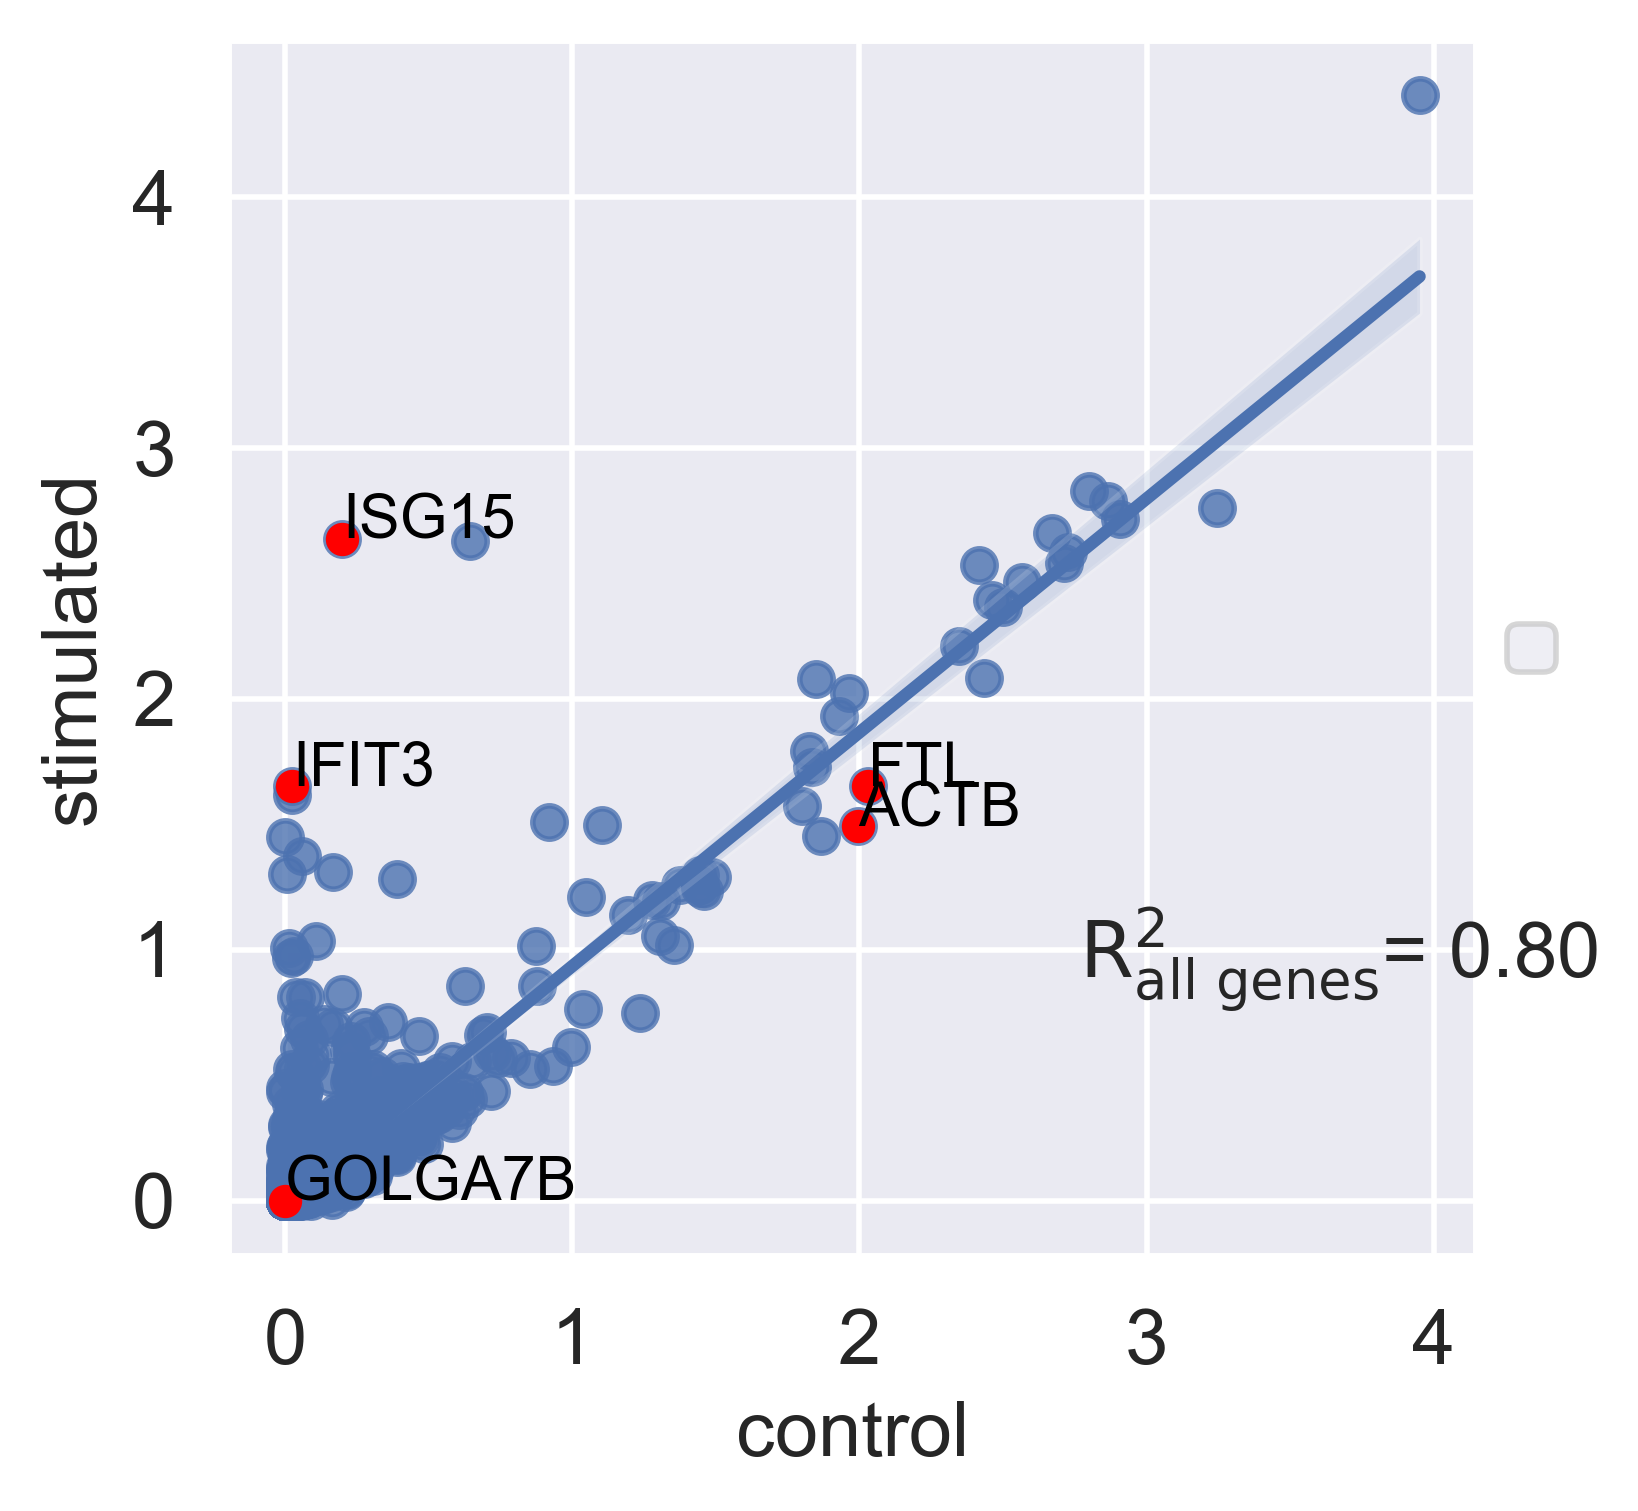
\includegraphics[width=0.7\textwidth]{images/Kang_bcells_ctrl_stim.png}
%\caption{
%B Cells mean expression regression, control vs stimulated.
%}
\label{fig:Kang_bcells_ctrl_stim}
\end{subfigure}
\begin{subfigure}[b]{0.49\textwidth}
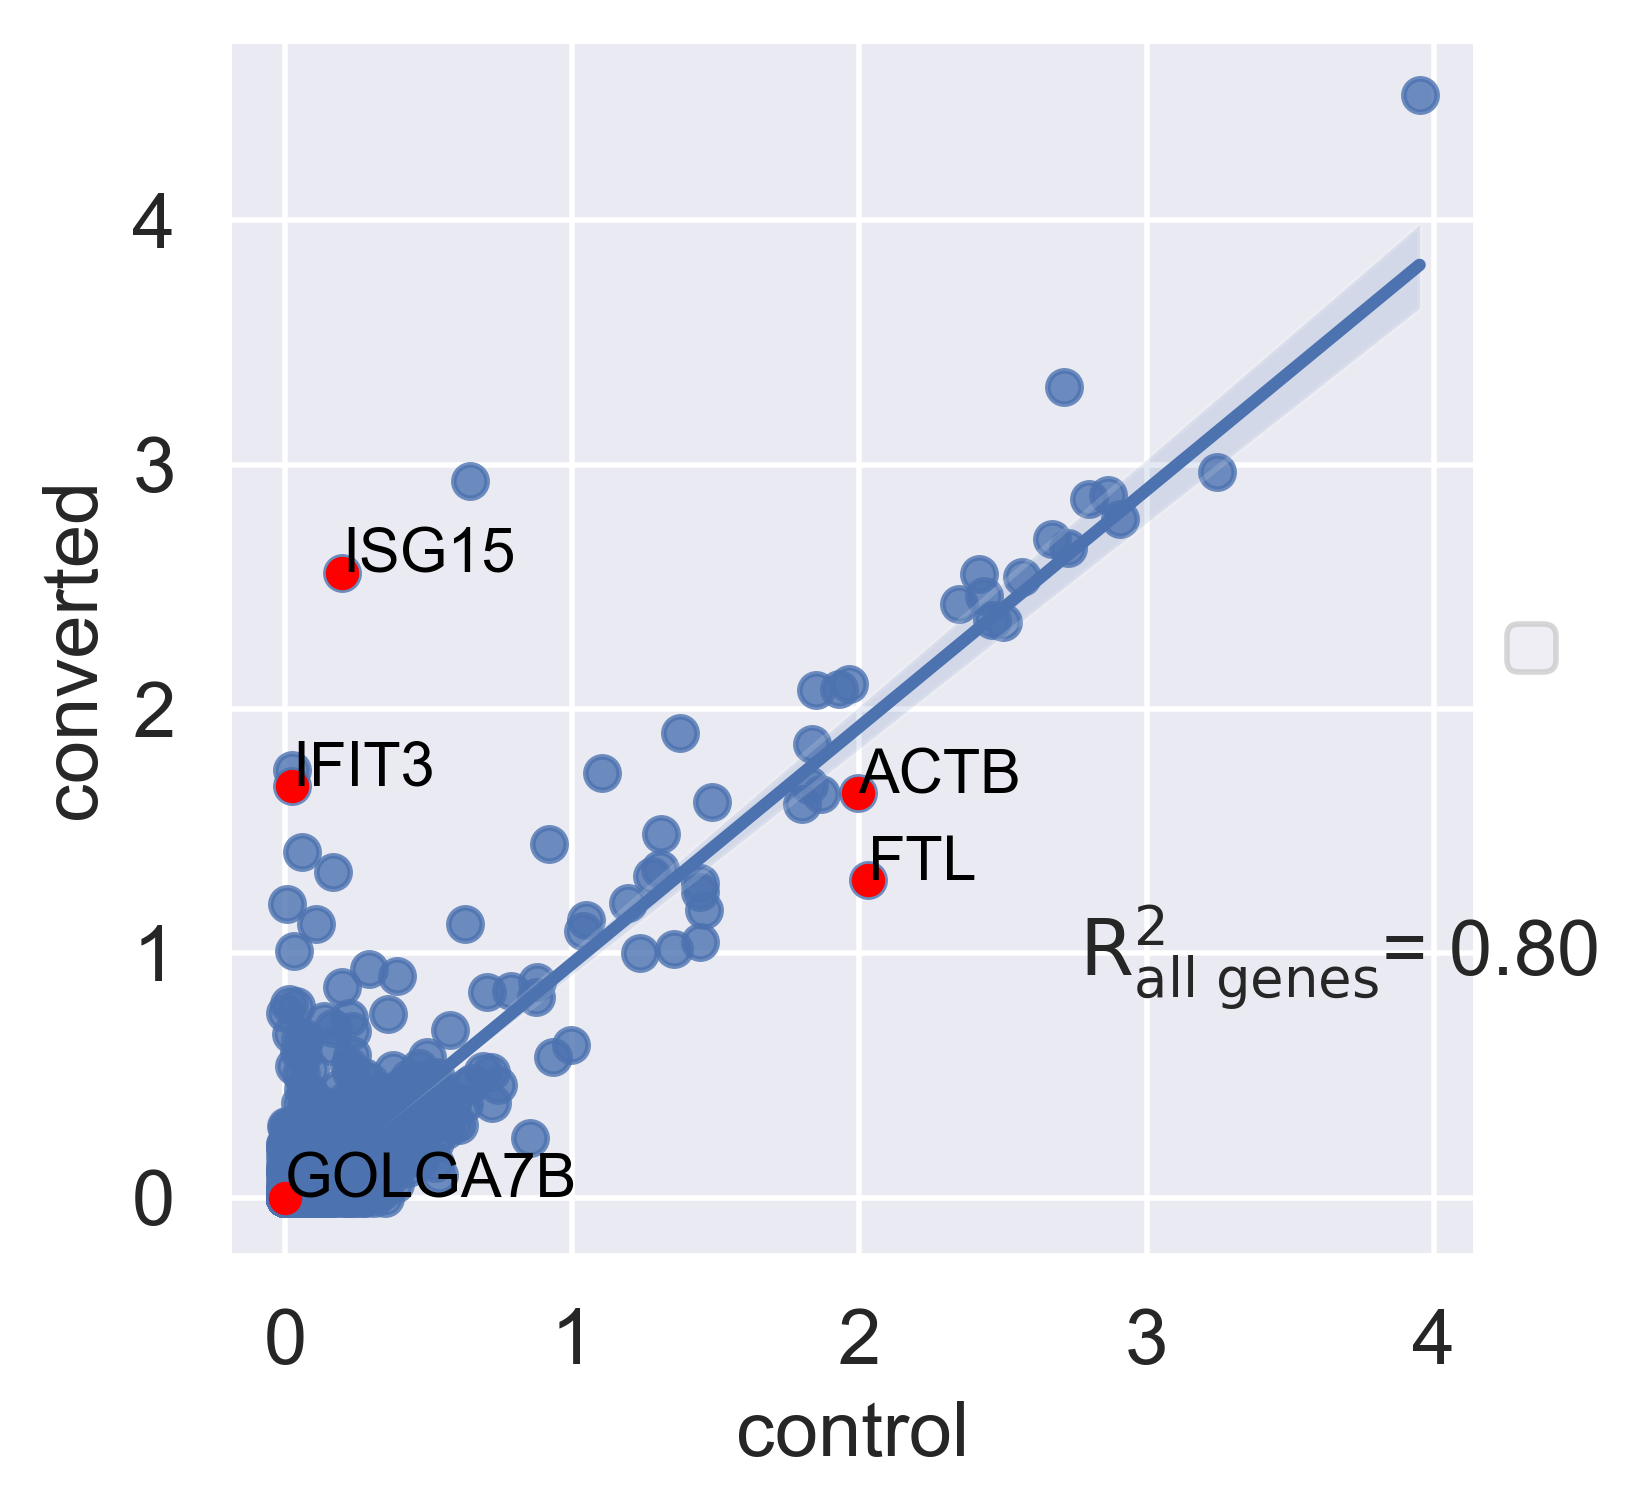
\includegraphics[width=0.7\textwidth]{images/Kang_bcells_ctrl_converted.png}
%\caption{
%B Cells mean expression regression, control vs
%control--converted--to--stimulated.
%}
\label{fig:Kang_bcells_ctrl_converted}
\end{subfigure}
\begin{subfigure}[b]{0.49\textwidth}
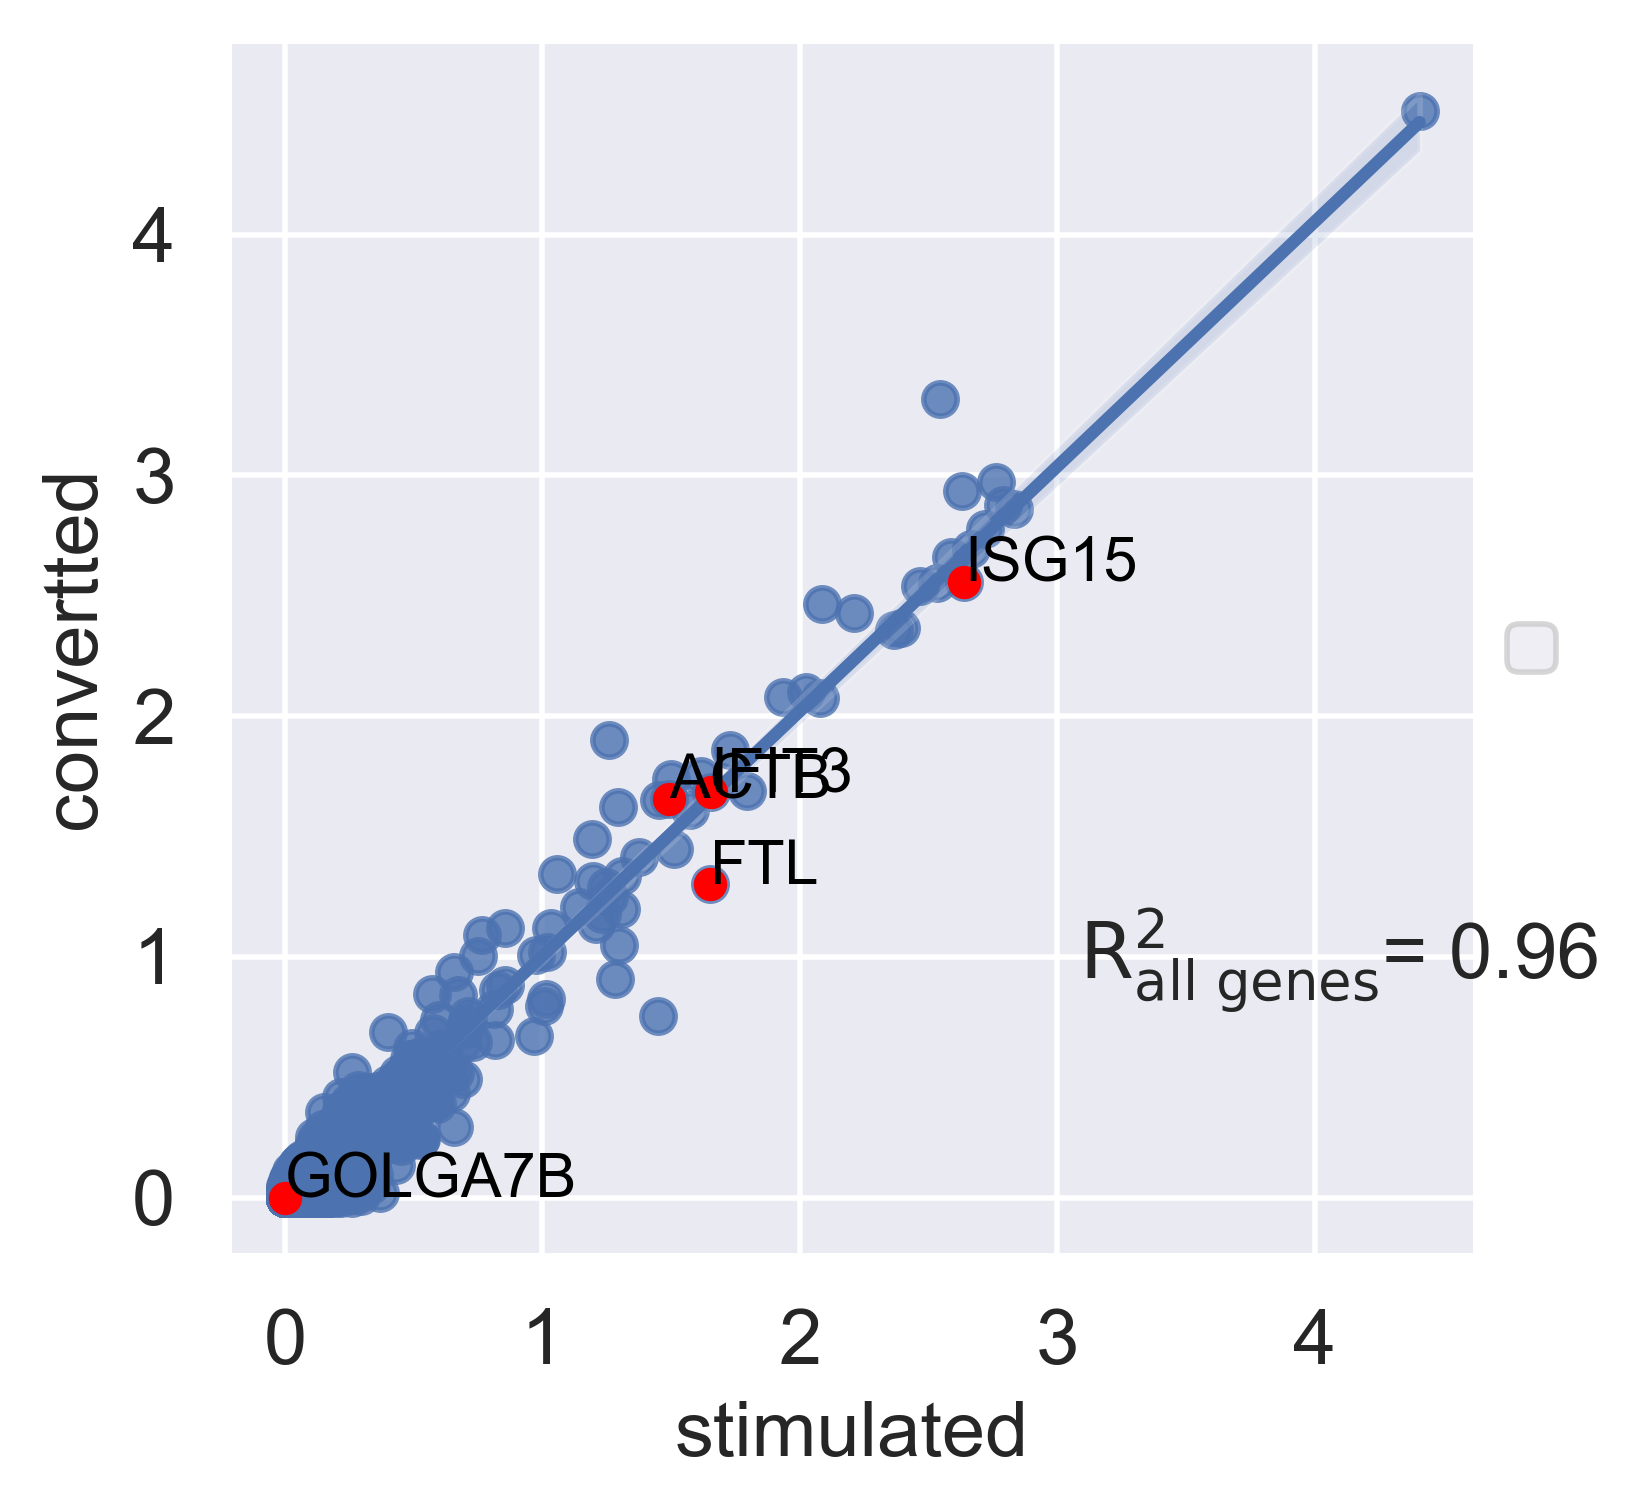
\includegraphics[width=0.7\textwidth]{images/Kang_bcells_stimulated_converted.png}
%\caption{
%B Cells mean expression regression, stimulated vs
%control--converted--to--stimulated.
%}
\label{fig:Kang_bcells_stimulated_converted}
\end{subfigure}
\end{figure}
\end{frame}

\begin{frame}
\frametitle{Generating data}
\begin{figure}[h]
\centering
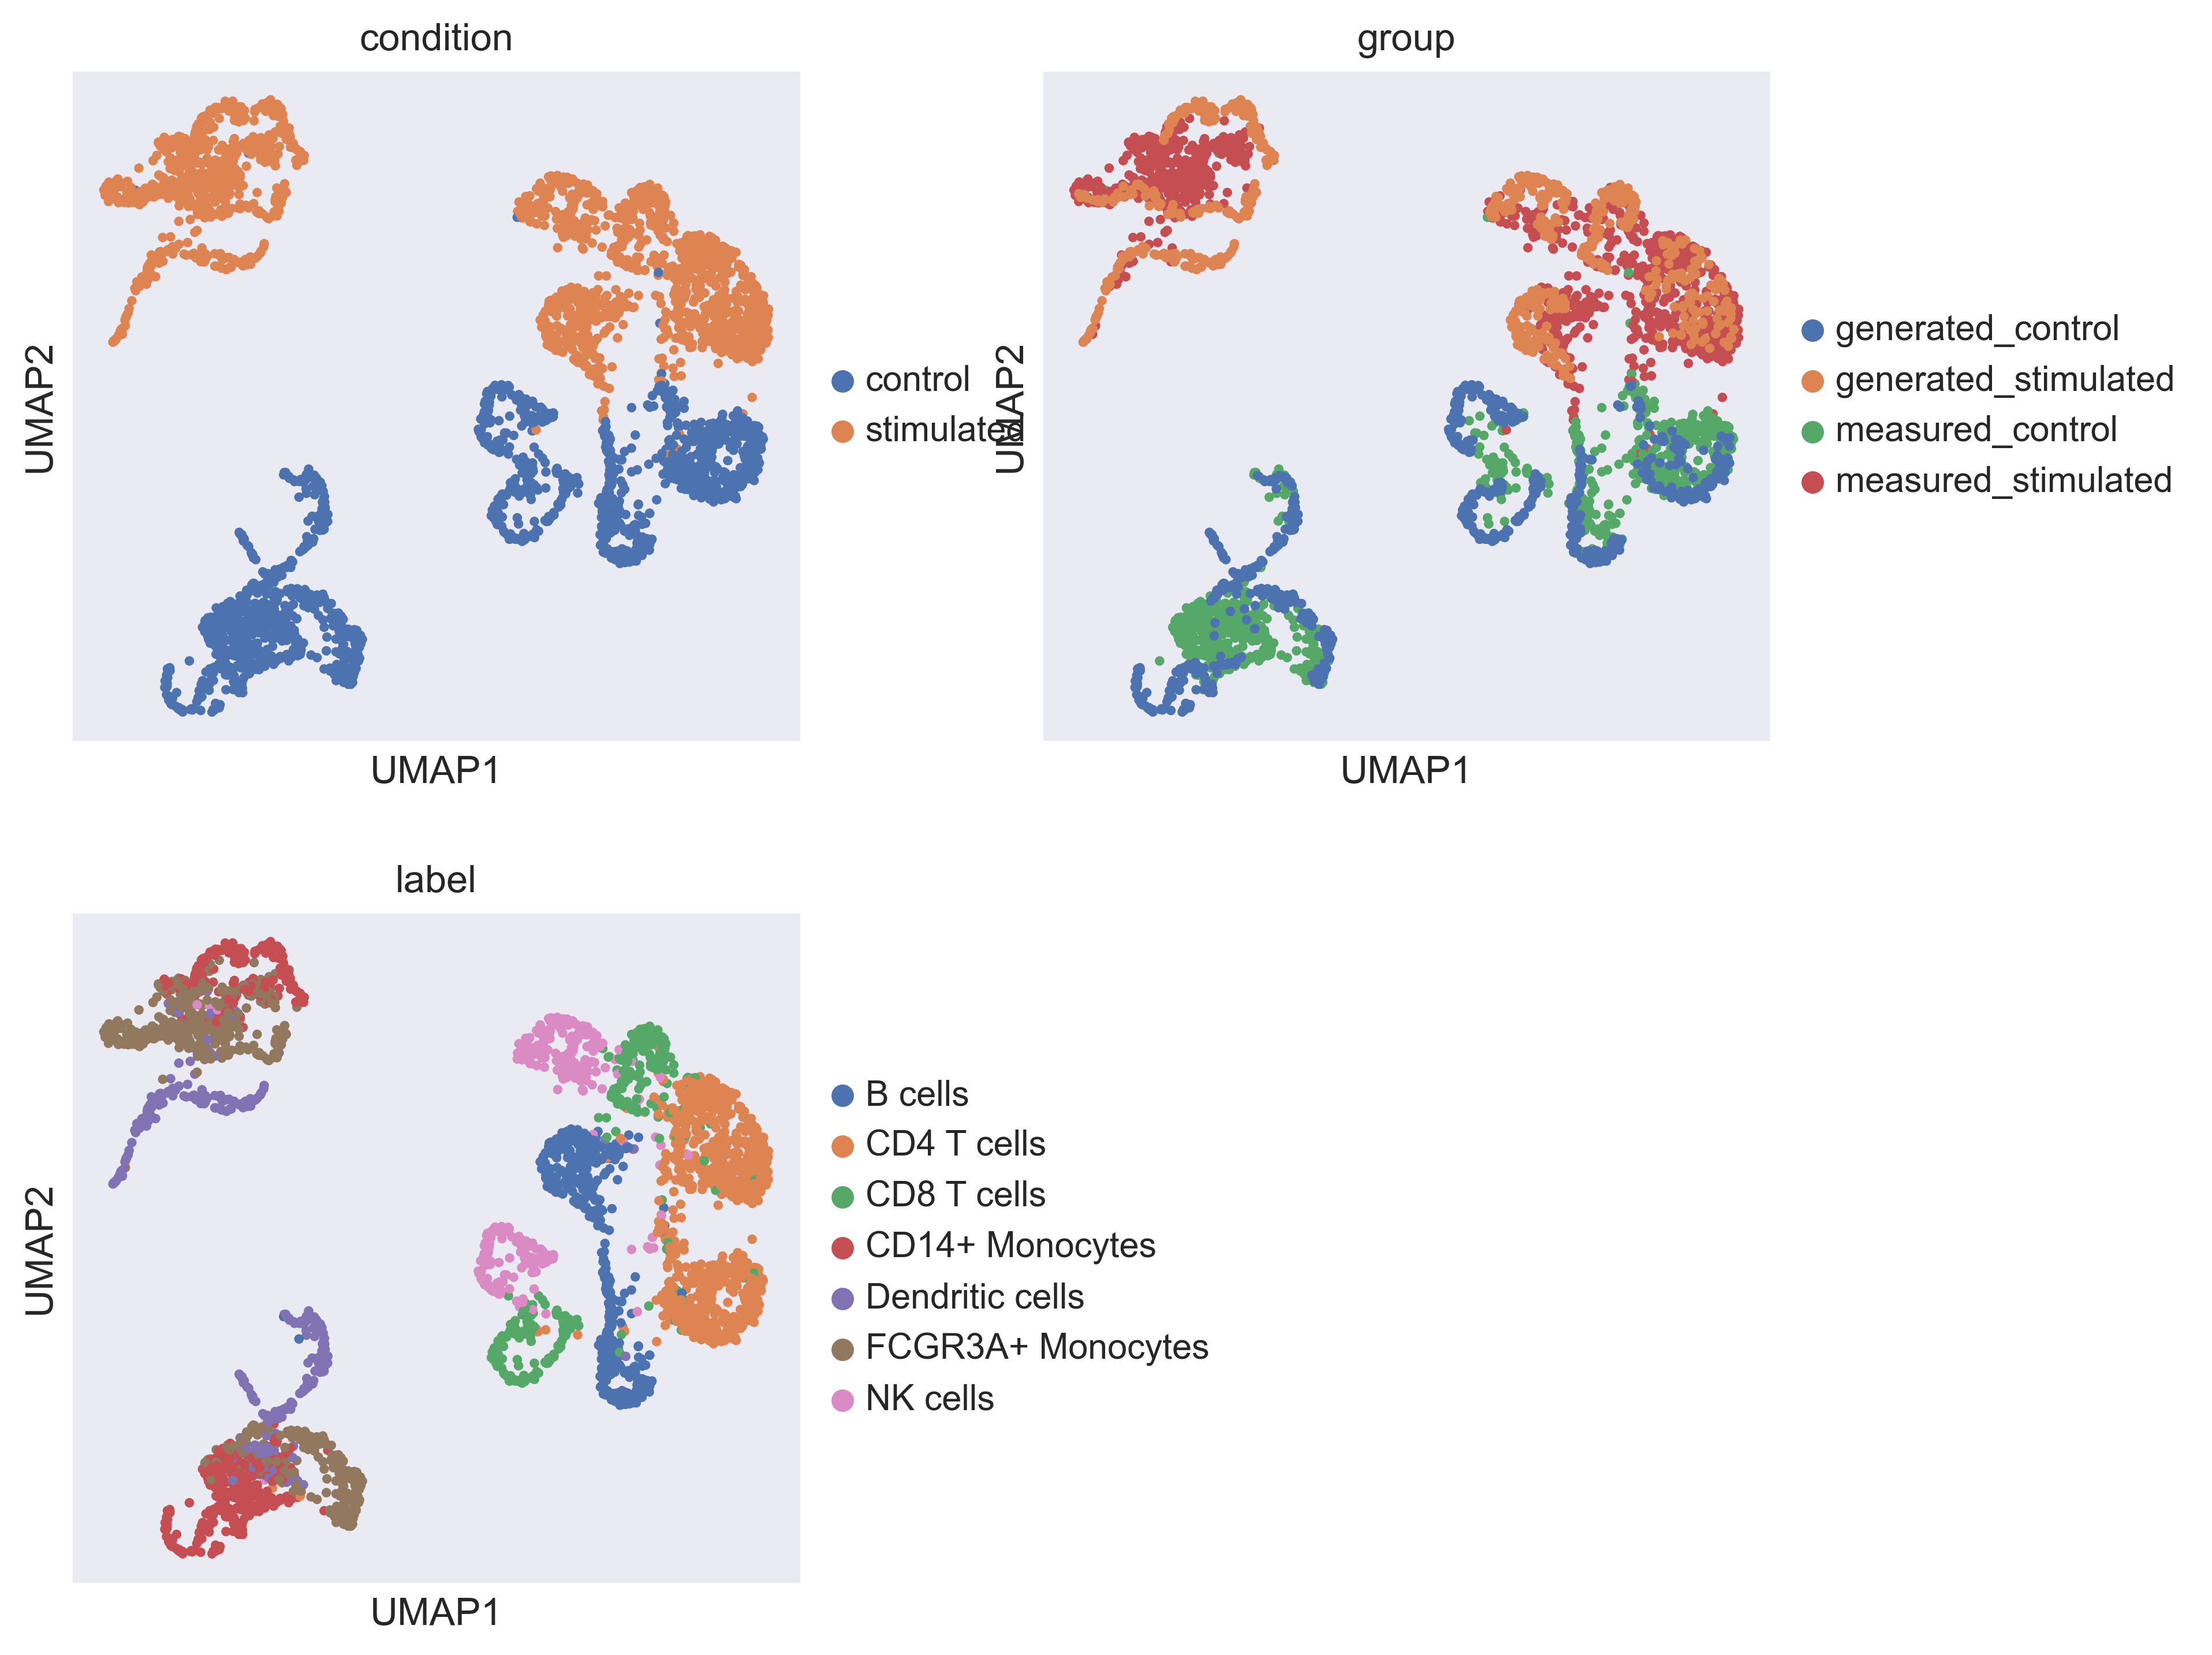
\includegraphics[width=0.85\textwidth]{images/Kang_generated_data.png}
\caption{
The Kang UMAP of real data combined with randomly generated data.
}
\label{fig:Kang_generated_data}
\end{figure}
\end{frame}


%\begin{frame}
%\frametitle{Spam}
%\begin{block}
%\maketitle
%\end{block}
%%\titlepage
%\begin{multicols}{2}
%Spam~\footfullcite{russkikh2020style} is good.
%spam spam spam
%\lipsum[1]
%\lipsum[2]
%\end{multicols}
%\end{frame}
%
%\begin{frame}
%\frametitle{Bigass equation}
%foo
%far
%\end{frame}

%\begin{frame}
%And now to something~\cite{guo2017improved} completely different \dots
%\end{frame}

\section{Reference}
%\begin{frame}
\nocite{bishop2006pattern}
\nocite{bishop2006pattern}
\nocite{kingma2014semi}
\nocite{dilokthanakul2016deep}
\nocite{lotfollahi2019scgen}
\nocite{mg22Repo}
\nocite{mpgvaeRepo}
\nocite{kingma2013auto}
\printbibliography
%\end{frame}

\begin{comment}
\end{comment}

\end{document}
